\chapter{面向时序结构识别的逆向师生蒸馏学习方法}

\section{问题的提出}



\subsection{波浪结构识别的量化难点与高频噪声干扰}

前两章分别从投资组合管理和高维金融因子建模角度讨论了资产配置与因子依据问题，但在真实交易过程中，资产和因子依据并不能直接转化为交易时点。即便某一资产具备配置价值，仍需进一步判断当前市场结构是否支持进场，以及趋势、反转或震荡状态是否具有交易意义。因此，本章进入对冲基金交易决策链条中的时序结构识别环节，以波浪结构识别作为具体切入点，研究如何在高噪声、非平稳的金融时间序列中识别趋势结构、结构边界与有效波段。

艾略特波浪理论由艾略特于20世纪提出，其核心观点是市场波浪运动遵循``五浪推进+三浪调整''的循环模式，并在不同时间尺度上递归嵌套，呈现较明显的分形特征。相关研究曾将艾略特波浪思想用于股票市场结构分析与推荐场景，说明该理论在刻画趋势延续和反转结构方面具有一定应用基础\cite{tirea2012stock}。不过，本文并不把波浪理论理解为人工划线规则的简单复用，而是借用其层级嵌套和趋势—调整结构视角，将其转化为可监督、可检验的时序结构识别问题。图~\ref{fig:placeholder}展示了艾略特波浪理论的基本结构，包括五浪推进与三浪调整的典型形态及其分形嵌套关系。

\begin{figure}[htbp]
    \centering
    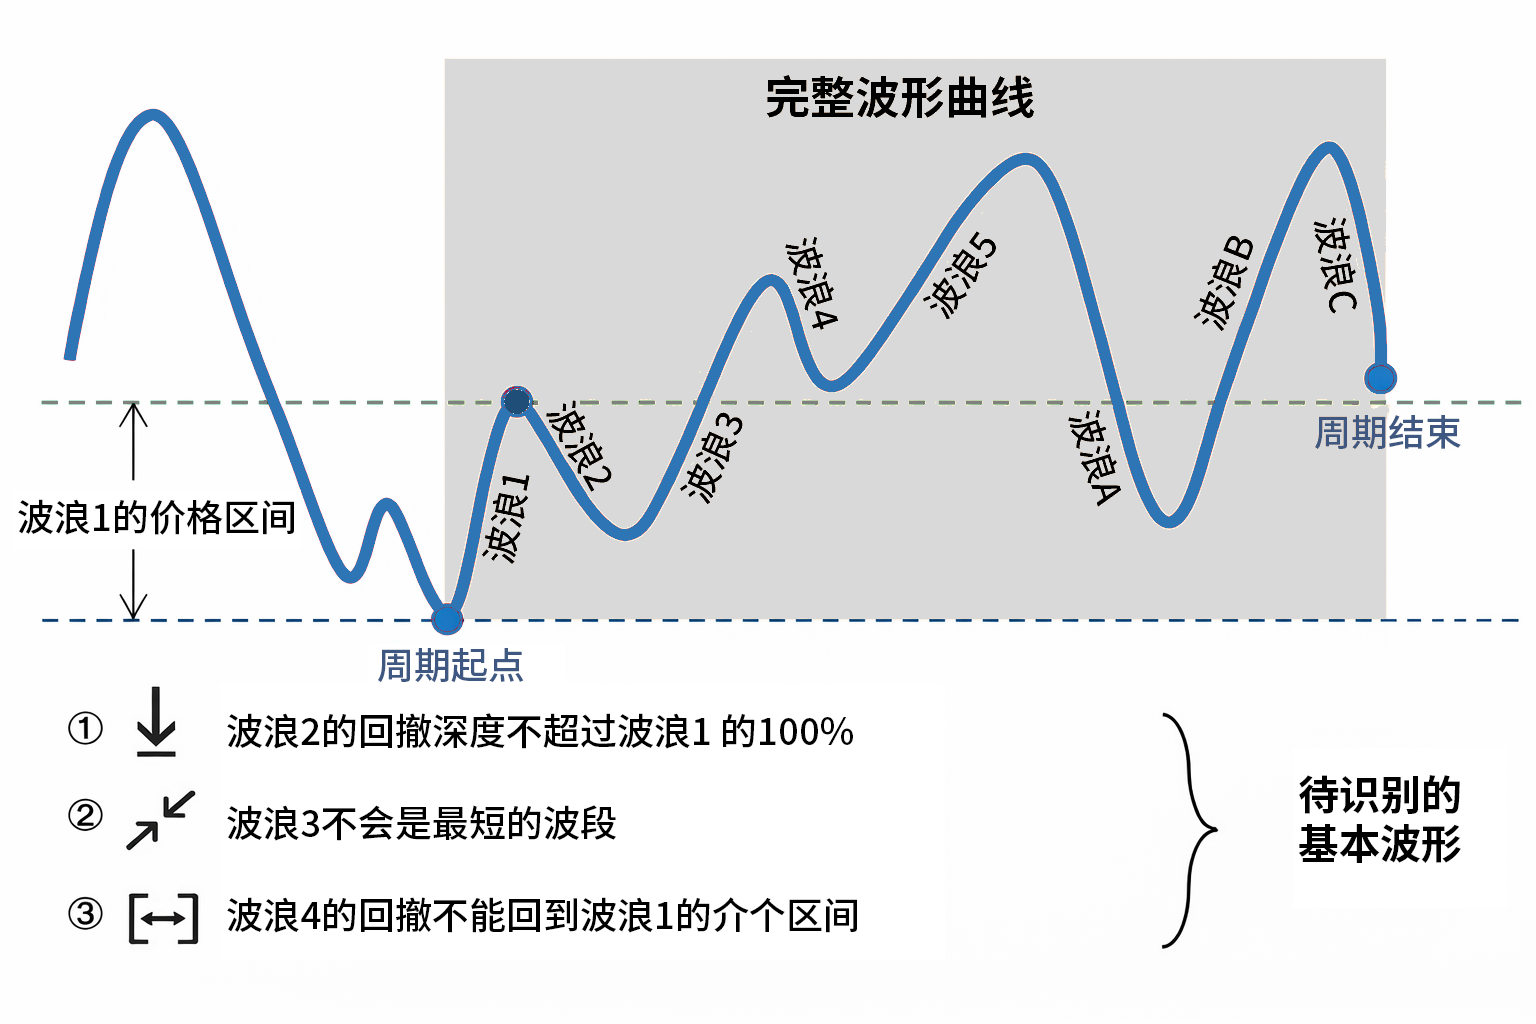
\includegraphics[width=1\linewidth]{figures/chap5/图4.1改.png}
    \caption{艾略特波浪理论}
    \label{fig:placeholder}
\end{figure}

在本章语境下，波浪结构被处理为金融时序结构的一种可操作化表达。交易时机判断不只取决于单一价格点位，还取决于价格路径是否已经形成相对稳定的趋势结构、转折结构或突破结构。然而，金融市场固有的高频噪声与结构模糊性会使部分局部波动被误识别为有效波段。高频交易与市场微观结构研究提示，噪声放大和短周期扰动会持续影响金融序列的可建模稳定性\cite{ba2019highfreq}。在这种环境下，传统依赖人工划分的波浪理论面临明显瓶颈：已有研究指出，波浪边界具有较强主观性，不同分析者之间的划分结果容易出现不一致\cite{wawer2024large}。

除人工划分差异外，波浪结构识别还受到市场状态变化本身的影响。经典区制转换模型表明，金融时间序列可能在不同市场状态之间切换，单一静态规则难以持续适配状态转移后的价格结构\cite{hamilton1989regime}。因此，波浪尺度会随着市场波动强度和状态转换过程动态变化，规则驱动方法即便在局部样本中有效，也难以长期保持稳定。

具体而言，波浪结构量化主要面临三类问题。第一，结构边界具有模糊性，同一段价格序列可能被划分为不同浪型；第二，波浪结构具有多尺度嵌套特征，需要同时识别推进浪、调整浪及其递归关系；第三，高频噪声会产生局部伪结构信号，使模型难以区分真实趋势转折与短暂价格扰动。因而，解决这一矛盾不能只停留在规则修补层面，还需要借助表示学习和结构校正机制对波浪边界进行更稳定的刻画。

数据驱动方法为金融时序建模提供了重要工具，但其有效性并不自动等同于波浪层级结构的稳定识别。金融深度学习研究说明，深度模型能够刻画复杂价格形成过程中的非线性关系\cite{sirignano2021universal}。但是，这类模型的主要目标通常是预测未来价格、收益方向或状态标签，而不是显式识别波浪边界、波段层级和结构转换位置。换言之，预测精度提高并不必然意味着模型已经理解了价格运动的层级结构。对于本章而言，关键问题不是继续证明深度模型能够进行价格预测，而是进一步说明如何把局部价格事件组织为结构清晰、边界可校正、具有交易含义的时序结构。

上述问题共同表明，金融时序结构识别不能被简化为一般价格预测或普通分类任务。金融资产收益序列普遍存在尖峰厚尾、波动聚集等经验特征，高频噪声与极端波动会进一步干扰局部结构识别\cite{Cont2001Empirical}。在这种数据环境下，模型即便在局部预测上有效，也未必能够形成稳定的层级结构表示。相关金融深度学习综述也表明，现有研究更多集中于直接价格预测或分类标签\cite{OZBAYOGLU2020106384}。因此，本章在一般深度预测模型之外，引入能够表达波浪结构、刻画局部事件边界并抑制高频伪结构干扰的标注与蒸馏机制，为后续四元分形事件识别和逆向师生蒸馏方法奠定问题基础。

\subsection{传统单向教师蒸馏范式在波浪结构识别中的局限性}

知识蒸馏由Hinton等人提出，主要通过教师模型向学生模型传递软标签或中间层表示，以改善模型泛化能力\cite{hinton2015distilling}。后续研究虽然将蒸馏方法扩展到多教师蒸馏、在线蒸馏和互学习等形式，但其基本逻辑仍多围绕教师模型向学生模型传递知识展开。不过，在波浪结构识别场景中，蒸馏机制面对的核心问题并不是学生模型能否模仿教师模型，而是教师模型的结构判断是否足够稳定、是否会把局部噪声误判为有效波段，并通过软标签传递给学生模型。

在时序结构识别任务中，蒸馏机制的作用不能仅理解为模型压缩。教师模型若对局部高频波动形成过度自信判断，学生模型会被迫继承这种偏差，最终导致结构边界识别不稳定。对于交易流程而言，这种偏差会表现为买入时机提前、滞后或误触发。因此，逆向师生蒸馏在提升模型泛化能力的同时，引入学生模型对复杂局部结构的反向校正，以降低单一强模型对伪趋势和噪声结构的误判。

多主体协同学习为这种反向校正提供了可借鉴的组织思路。多智能体系统强调多个学习主体之间的协作、竞争与信息共享，有助于在非平稳环境中形成更具适应性的策略\cite{lee2007multiagent}。但是，已有多主体方法并不能直接解决波浪结构识别中的边界模糊和类别不平衡问题。对本章而言，多主体协同的价值主要体现在允许不同模型对同一局部结构形成差异判断，并利用这种差异约束教师模型的过度自信输出，而不是简单增加模型数量。

进一步看，多智能体强化学习相关综述强调，多主体学习并不只依赖单个最优策略，而是通过多个学习主体在共享环境中的交互来提升复杂环境适应性\cite{du2019survey}。这一思路对本章的启发在于，波浪结构识别中的不同模型判断应当被用于相互校验，而不应让单一教师模型长期垄断结构边界定义。

同时，单向教师蒸馏还可能强化强模型主导下的结构偏差。生成对抗网络研究中的模式坍缩概念提示，在对抗或博弈式训练过程中，模型输出可能逐渐收缩到少数优势模式\cite{goodfellow2014generative}。在金融时序结构识别中，类似风险表现为：强模型在训练后期逐渐主导结构判断，使弱模型难以保留对少数类、极端波动或局部反转结构的探索能力，最终造成结构表达退化。常规``教师到学生''的单向机制在金融市场这种高度非平稳环境中，缺乏必要的自我纠错能力。

从信息传递角度看，传统蒸馏中的软标签虽然包含类间关系信息，但这种信息传递通常是单向且相对静态的。知识蒸馏综述也表明，蒸馏知识可以来自响应输出、中间特征和样本关系等不同层次\cite{gou2021knowledge}。这一点说明，蒸馏机制本身具有较强的扩展空间，但在市场剧烈波动期间，教师模型仍可能对某类波浪结构产生系统性偏差；学生模型如果过度拟合教师输出，就难以通过自身探索发现更准确的结构边界。因此，本章强调的逆向师生蒸馏并不是简单让弱模型反过来替代强模型，而是在结构识别误差出现时，将学生模型捕捉到的局部差异作为反向约束信号，用于修正教师模型对伪结构和边界位置的误判。

基于上述分析，本章需要解决的关键问题可以进一步凝练为三个层次：第一，如何将具有主观解释色彩的波浪形态转化为边界清晰、可重复标注的结构事件，使趋势结构识别具备可监督训练基础；第二，如何在强噪声和类别不平衡条件下抑制强模型对局部伪结构的过拟合，使结构边界识别不被单一高置信度判断锁定；第三，如何判断已识别的结构信号是否能够延续为具有交易意义的有效波段，从而真正服务于交易流程中的交易时机判断。因此，本章并不把目标设定为单纯提高价格方向预测精度，而是围绕``结构可量化、边界可校正、信号可交易''构建时序结构识别方法。后续方法设计中，四元分形事件主要回应结构量化问题，逆向师生蒸馏主要回应边界校正与噪声抑制问题，带鱼短鱼机制则用于补充趋势有效性判别。



\section{相关工作}

围绕金融时序结构识别，已有研究大体可以分为三类：一是以波浪理论和技术形态分析为代表的结构解释方法，二是以深度序列模型、注意力机制和生成式建模为代表的数据驱动识别方法，三是以知识蒸馏和多模型协同为代表的泛化提升与误差校正方法。这些研究分别从市场形态、序列表示和模型迁移角度提供了有益基础，但与本文关注的交易时机识别任务相比，仍存在结构边界不清、局部噪声干扰、预测输出难以回到波浪层级以及单向知识传递容易放大教师偏差等问题。因此，本节并不把相关工作简单归纳为价格预测或模型分类问题，而是围绕“结构能否被清晰标注、边界能否被稳定校正、识别结果是否具有交易延续性”三个方面展开讨论。

传统波浪理论强调价格运动中趋势推进与调整回撤的层级关系，为观察金融序列的结构性变化提供了直观框架。相关实证研究也尝试检验艾略特波浪理论在金融市场预测中的有效性\cite{dangelo2017effectiveness}。这说明波浪理论具有一定的市场解释价值，但其应用过程往往依赖人工识别和经验划分。对于可重复训练的深度学习框架而言，真正困难的并不是确认市场中存在某种形态经验，而是将波浪起止点、层级嵌套关系和有效波段边界转化为可监督、可回溯且可在不同样本中重复执行的结构事件标签。

深度时序模型为金融序列中的趋势识别和状态判别提供了新的工具。股票价格预测研究表明，循环神经网络类模型能够从高噪声价格序列中提取局部时序模式\cite{nelson2017stock}。这类研究为金融序列建模提供了数据驱动基础，但其目标通常是价格拟合或方向预测，模型输出并不会自动对应波浪边界。对于本章任务而言，预测曲线是否贴近真实价格只是一个中间问题，更关键的是模型能否判断局部转折是否构成有效结构、识别出的结构能否延续为具有交易意义的波段。

近年来，长短期记忆网络仍被用于刻画金融趋势变化中的时间依赖关系\cite{xie2025lstm_trend}。这一方向说明门控循环结构在处理局部趋势变化时仍有价值，但单一序列模型容易把短期波动误认为趋势变化，也可能忽略波浪结构中的层级关系。进一步的混合时序模型研究则表明，将循环结构与其他深度模块结合，可以增强模型对复杂金融序列的表达能力\cite{ma2025transformer_lstm}。不过，表达能力增强并不必然意味着结构识别能力增强；如果缺少结构化标签和边界校正机制，模型仍可能在高频噪声、局部反转和短周期震荡中学习到伪结构。

在结构识别相关任务中，已有研究开始将深度序列模型用于股票状态类别识别\cite{wang2025lstm_classification}。状态分类把连续价格序列转化为离散市场状态，有助于缩小预测任务与交易判断之间的距离。与此同时，注意力机制与长短期记忆网络结合的研究表明，模型可以通过关注关键时段特征来改善金融序列状态判别\cite{li2024attention_lstm}。这类研究进一步说明，数据驱动模型已经能够从金融序列中提取部分趋势、状态和局部变化信息；但波浪结构识别不仅要求模型判断“处于何种状态”，还要求模型回答结构边界在哪里、局部反转能否延续、信号是否能够转化为可交易波段等问题。

生成式金融序列建模从另一侧拓展了时序结构研究。近期金融时间序列生成研究表明，生成式模型可以用于补充样本分布和模拟复杂市场状态\cite{vuletic2024fin}。这类工作对于缓解金融样本有限、市场状态覆盖不足等问题具有启发意义，但生成或补充数据本身不能直接解决波浪边界识别问题。若缺少结构化标签、边界校正和趋势有效性判别，生成模型仍可能在局部波动中放大伪结构，甚至把统计上相似但交易含义不同的片段混为一类。

国内相关研究也将生成对抗网络用于金融数据生成任务，为复杂金融序列分布建模提供了参考\cite{cui20241gan}。此外，深度生成模型被引入因子投资建模场景，说明生成式方法在金融表征学习中具有一定拓展空间\cite{ma2022deep}。这些研究共同说明，生成式方法能够服务于金融数据分布表达和样本扩展，但其作用仍主要体现在表征和数据层面。对于本文的波浪结构识别任务而言，仍需要进一步回答结构标签如何构建、类别不平衡如何处理，以及局部结构是否具有后续交易延续性等问题。

知识蒸馏和多模型协同方法为模型压缩、泛化提升和知识迁移提供了重要路径。相关知识蒸馏研究表明，蒸馏方法已经从单一教师—学生压缩范式扩展为多种知识迁移与模型协同形式\cite{huang2022distillation}。这一方向为本文引入逆向师生蒸馏提供了方法背景，但传统蒸馏更多强调强模型向弱模型传递知识，并未充分讨论学生模型对教师模型结构判断的反向校正作用。对于金融时序结构识别而言，强模型可能在局部噪声中形成过度自信的结构判断，若学生模型只能被动模仿，就可能继承这种偏差。因此，本章关注的不是一般意义上的模型压缩，而是利用模型间差异对强模型的结构边界判断进行反向约束。

基于上述不足，后文以波浪结构作为时序结构识别的具体场景，在四元分形事件标注方法的基础上，引入逆向师生蒸馏机制以提升结构识别的稳定性。与传统``强教师指导弱学生''的单向蒸馏不同，该机制强调当学生智能体在特定复杂结构上实现阶段性超越时，教师模型也应参考学生模型捕获的新分布特征，从而缓解强模型对局部高频噪声的过拟合问题。由此，相关工作所暴露出的主观标签、噪声干扰和单向蒸馏局限，构成了本章后续算法设计的直接动因。下一节将围绕结构标签构建、逆向师生蒸馏和趋势有效性判别三个层面展开方法设计。

\section{逆向师生蒸馏方法}

本节介绍面向时序结构识别的逆向师生蒸馏方法，并按照前文提出的三个问题展开。首先，针对波浪结构主观性强、边界不清的问题，通过四元分形事件将价格序列中的转折、交叉和突破结构转化为可监督标签；其次，针对强模型容易被局部噪声误导的问题，通过逆向师生蒸馏机制在多模型之间传递误差信息与结构边界信息，抑制强模型对局部伪结构的过拟合；最后，针对结构信号是否真正具有交易意义的问题，通过带鱼短鱼机制判断已识别结构能否延续为有效趋势。上述设计共同服务于交易流程中的交易时机判断，使结构信号从形态描述进一步转化为交易时机判断依据。

为避免将本章方法理解为单一分类模型，本节先从整体组织架构和任务设置两个层面说明方法设计。图\ref{fig:S2T-arch}展示了本章方法的三层组织结构：第一层将波浪结构转化为四元分形事件标签，第二层通过生成器组和判别器组构成逆向师生蒸馏系统，第三层将结构识别结果映射到分类与交易应用。图\ref{fig:S2T-task}进一步说明四元分形事件在多任务预测中的组织方式，为后续4.3.1的标签定义、4.3.2的模型构建和4.3.3的逆向蒸馏机制提供任务入口。

\begin{figure}[!htbp]
    \centering
    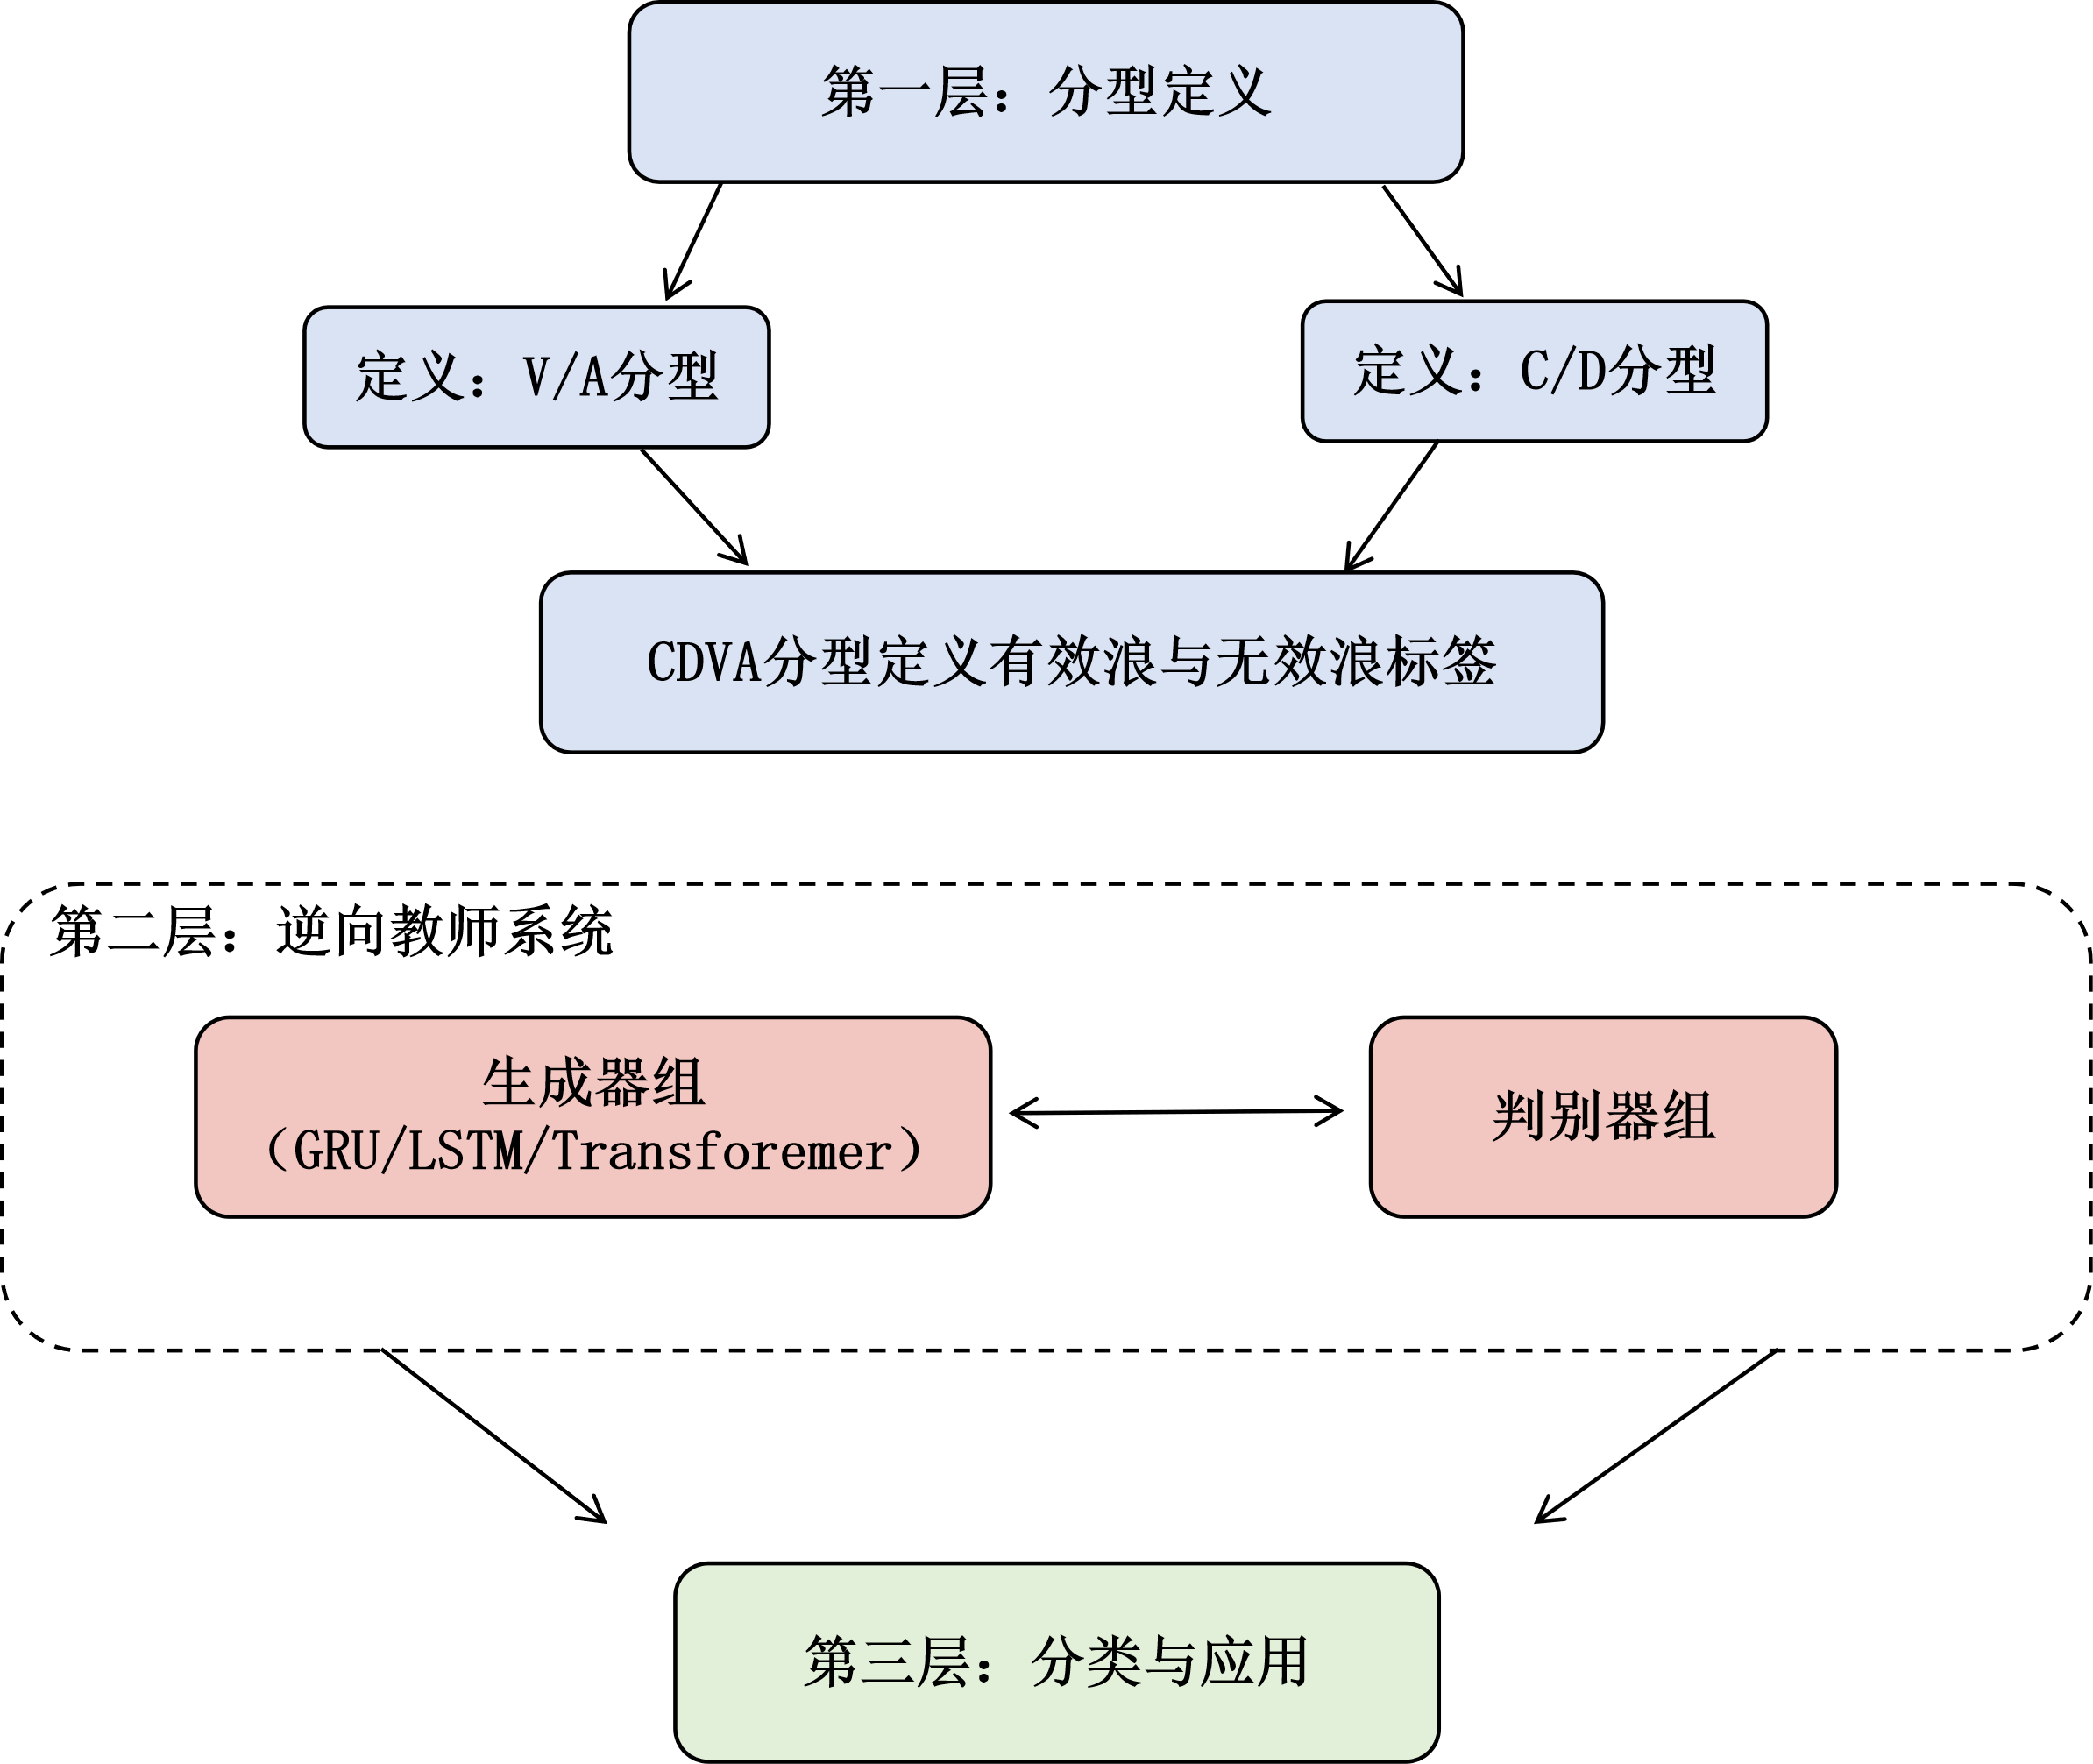
\includegraphics[width=0.8\textwidth]{figures/chap5/波浪架构.png}
    \caption{基于逆向师生蒸馏机制的时序结构识别组织架构}
    \label{fig:S2T-arch}
\end{figure}

\begin{figure}[!htbp]
    \centering
    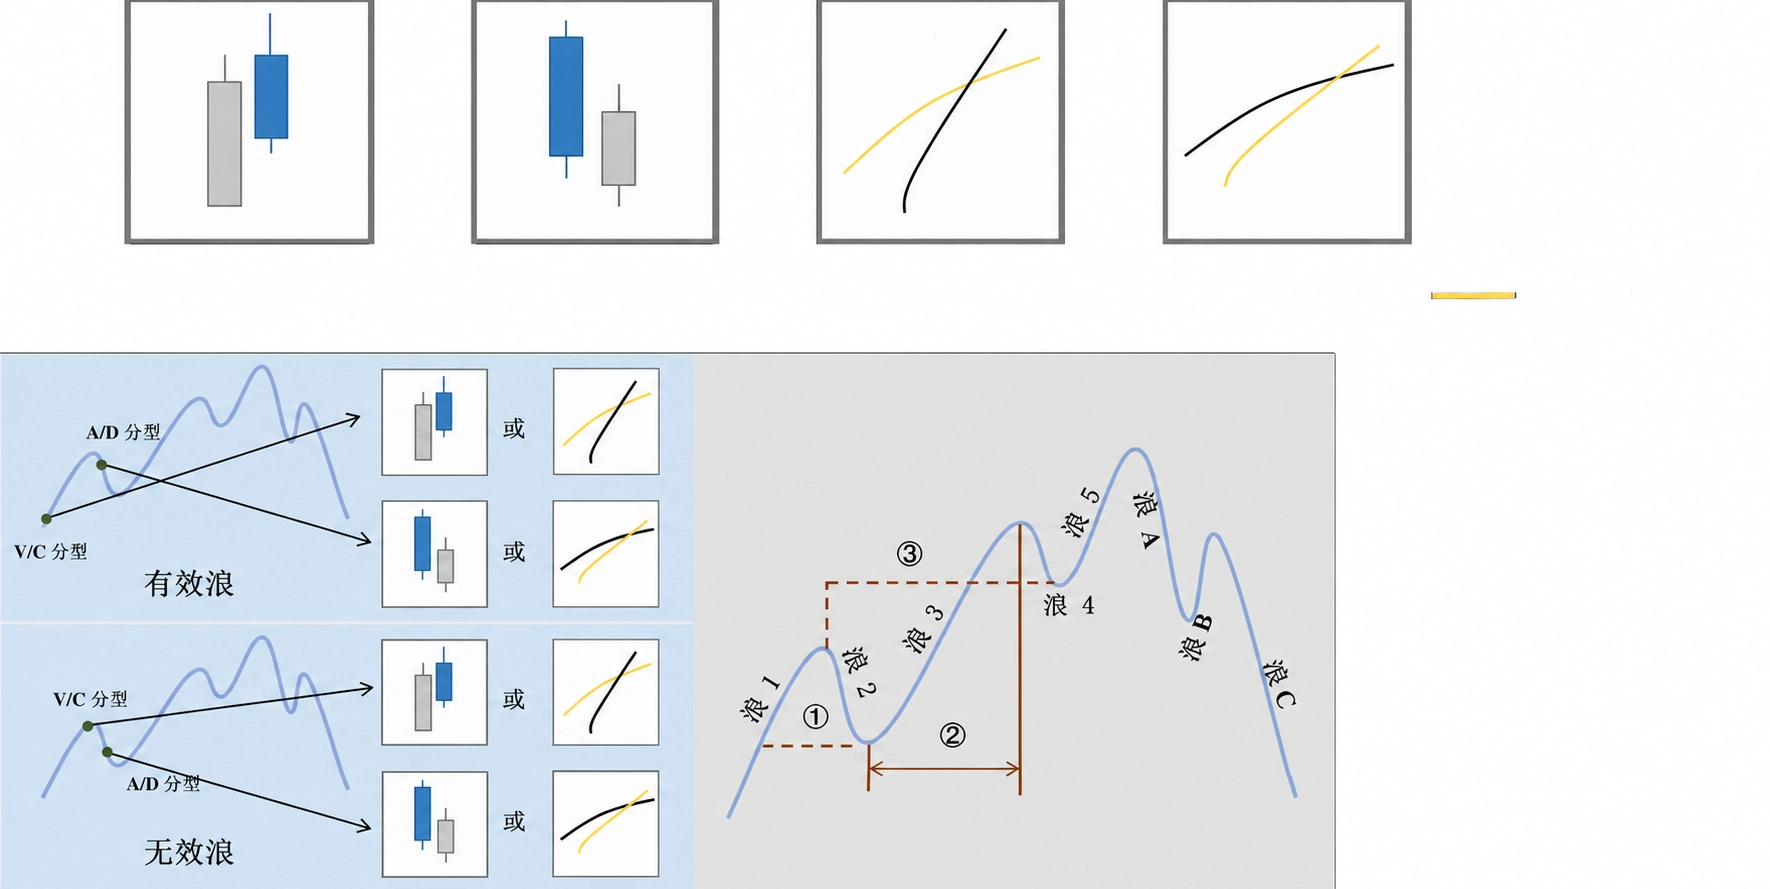
\includegraphics[width=0.8\textwidth]{figures/chap5/图4.3改.png}
    \caption{基于逆向师生蒸馏机制的时序结构识别任务}
    \label{fig:S2T-task}
\end{figure}

\clearpage

\subsection{四元分形事件标注方法与波浪结构量化重构}

``裸K线交易法''强调在交易图表中剔除均线、指数平滑异同移动平均线、布林带等衍生指标，仅依据原始K线（蜡烛图）的形态、组合排列及关键支撑阻力位分析市场微观结构。这类方法直观、贴近交易实践，但其判断过程很大程度上依赖视觉经验，长期缺乏可重复的数学边界。与之相对，传统深度学习模型虽然能够处理连续价格序列，却往往把价格变化压缩为浮点数张量，弱化了K线之间最基本的拓扑排列关系，使结构判定与模型输出之间缺乏直接对应。

基于这一问题，本章提出四元分形事件标注方法。其中，V（向上突破）与 A（向下跌破）分型对应于相邻K线之间最基础的突破与跌破结构。此类将交易经验规则转化为可计算结构标签的思路，与国内关于金融数据生成建模和结构化表示学习的研究取向具有一致性\cite{xu2024gan}。通过对前一周期实体边界与当前收盘价之间的关系进行明确刻画，原本依赖经验识别的K线排列被转化为可重复的二元事件标签。这样处理的目的，不是简单增加一组技术指标，而是为后续模型训练提供结构化输入，并使输出结果能够回到原始K线图上进行解释。换言之，四元分形事件标注方法试图在裸K线经验与深度模型之间建立可计算的对应关系，使模型识别结果具有较清楚的图形解释基础。

四元分形事件在本章中的作用，是将原本主观的波浪划分转化为可重复的时序结构标签。C/D事件刻画动量结构的方向切换，V/A事件刻画价格实体的局部突破与跌破，它们共同提供了趋势启动、趋势反转和结构确认的候选时点。因此，该标签体系不仅用于形态分类，也为交易时机判断提供可监督的结构化输入。

为了构建可用于深度模型训练的结构化波浪标签体系，本章基于动量类指标与K线结构行为，设计了四元分形事件：C（上穿）、D（下穿）、V（向上突破）、A（向下跌破）。相比传统波浪结构定义，该体系更易量化，边界也更便于在大规模时序数据上重复标注。四元分形事件的设计遵循两个原则：其一，C与D基于动量指标的方向切换，捕捉趋势的宏观转折信号；其二，V与A基于K线实体的价格突破，捕捉微观层面的结构性波动。这种宏观与微观相结合的标签设计，使得模型能够在多个时间尺度上同时学习波浪结构特征。

在构建C（上穿）与D（下穿）两类方向性切换分形时，本章引入了指数平滑异同移动平均线。指数平滑异同移动平均线由快速与慢速两条指数加权移动平均线构成，二者之差定义为动量线：

\begin{equation}
\mathrm{DIF}_t = \operatorname{EMA}_{\text{fast}}(P_t) - \operatorname{EMA}_{\text{slow}}(P_t),
\end{equation}

其中$P_t$为时刻t的收盘价。动量线的指数移动平均为信号线，二者之差称为柱状线：

\begin{equation} \mathrm{DEA}_t = \operatorname{EMA}_{\text{signal}}(\mathrm{DIF}_t) \label{eq:dea} \end{equation}

\begin{equation} \mathrm{MACD}_t = 2 \times (\mathrm{DIF}_t - \mathrm{DEA}_t) \label{eq:macd} \end{equation}

本章将指数平滑异同移动平均线重新解释为``分形结构触发器''：当动量线由下向上穿越信号线时记为C（金叉）；当动量线由上向下穿越信号线时记为D（死叉）。相比传统手工波浪划分，这种基于指数平滑异同移动平均线的结构事件更具可量化性、鲁棒性与可重复性。需要指出的是，指数平滑异同移动平均线本身作为滞后指标，其信号触发时间通常晚于价格的实际转折点，这一特性在后续的``带鱼短鱼''机制中将被进一步讨论与补偿。

在方向性切换分形的基础上，本章进一步定义基于K线实体突破的结构性波动事件（V/A）。给定上一周期实体上沿与下沿：

\begin{equation}
U_{t-1} = \max(\mathrm{open}_{t-1},\, \mathrm{close}_{t-1}),
\qquad
L_{t-1} = \min(\mathrm{open}_{t-1},\, \mathrm{close}_{t-1}),
\end{equation}

则当前周期的V/A信号定义为：

\begin{equation}
V_t = \mathbb{I}(\mathrm{close}_t > U_{t-1}),
\qquad
A_t = \mathbb{I}(\mathrm{close}_t < L_{t-1}).
\end{equation}

V描述价格向上穿越前实体上沿的``结构性突破''，常对应趋势波段的延续；A描述价格向下跌破前实体下沿的``结构性回落''，常预示反转或加速回撤。V/A的定义基于严格的价格边界，对噪声不敏感，可在高频/日频数据上稳定复现。与C/D分形相比，V/A分形具有更高的时间分辨率，能够在趋势内部捕捉到更细粒度的结构变化，为模型提供了互补的多尺度结构信息。

基于上述定义，四元分形标签体系将波浪结构识别转化为可重复的监督信号，并为后续 4.3 节的模型构建与 4.4 节的实验比较提供统一的结构标签基础。更重要的是，该标签体系使时序结构识别能够与交易时机判断建立直接联系：结构事件的出现对应潜在买卖时点，结构事件的持续与反转则决定该时点是否具备进一步交易价值。由此，四元分形事件在本章中不是附加的技术指标集合，而是把传统波浪形态转化为可学习结构输入的关键环节，直接回应了 4.1 节提出的结构量化问题。

\subsection{逆向师生蒸馏的误差信息传递与反向校正}

本节在四元分形事件标注方法的基础上，也说明逆向师生蒸馏机制如何服务于时序结构识别。与一般分类模型只关注标签预测不同，本节关注的是在高噪声、非平稳金融序列中，如何通过模型间误差信息传递抑制局部伪结构，使强模型在追求低损失的同时仍受到组内结构分布约束。由此，逆向师生蒸馏在本章中主要承担结构边界识别、噪声过滤与交易时机确认中的训练约束作用，而不只是模型压缩工具。

\noindent\textbf{状态空间构建与特征提取优化}\par

在明确了C、D、V、A四元分形事件的边界与触发条件后，本章将波浪结构识别转化为一个基于多变量时间序列的多任务学习问题。给定长度为T的金融时间序列$X = \{x_1, x_2, \dots, x_T\}$，其中$x_t \in \mathbb{R}^d$表示t时刻的d维特征向量，时间窗口大小为W，模型在t时刻的输入为$X_{t-W+1:t} \in \mathbb{R}^{W \times d}$。本章的任务目标是学习一个深度映射函数$f_\theta$，预测目标空间包含两部分：结构分类标签$y_t$ = ($y^C_t, y^D_t, y^V_t, y^A_t$)属于$\{0, 1\}^4$，其中$y^k_t = 1$表示第k类分形事件发生；结构持续时间$l_t$ = ($l^C_t, l^D_t, l^V_t, l^A_t$)$\in \mathbb{R}^4$，表示对应分形结构从触发到结束的时间跨度。整体任务形式化为：

\begin{equation}
    (\hat{\mathbf{y}}_t, \hat{\mathbf{l}}_t) = f_\theta(\mathbf{X}_{t-W+1:t})
\end{equation}

其中$\hat{y}_t \in [0, 1]^4$为各分形事件发生的预测概率，$\hat{l}_t$为预测的持续时间。通过这一形式化定义，传统波浪理论中主观、模糊的``形态识别''过程被严格转化为可端到端优化的多标签分类与回归联合预测任务。

在时序结构识别任务中，误差信息不仅表示分类错误，也反映模型对结构边界、趋势转折和局部噪声的判断偏差。逆向师生蒸馏的意义在于，当弱模型在某些局部结构上保留了更丰富的边界信息时，强模型可以通过反向校正避免过度收敛到单一高置信度判断，从而提升对复杂时序结构的识别稳定性。该机制对应 4.1 节提出的第二类问题，即传统单向蒸馏容易把强模型偏差传递给弱模型，导致交易时机判断提前、滞后或误触发。

\noindent\textbf{逆向师生蒸馏机制的核心逻辑与误差信息传递}\par

本章构建了由多生成器（预测网络）与多判别器（结构校验网络）组成的训练框架。生成器组由门控循环单元、长短期记忆网络与自注意力序列模型三类异质网络构成，以实现``局部短期记忆-全局长程依赖''的特征互补。自注意力序列模型生成器采用4层编码器结构，多头注意力机制的头数设为8，隐藏层维度为256；门控循环单元与长短期记忆网络生成器均采用双层堆叠结构，隐藏层维度设为128。判别器组由多层感知机与对应时序网络构成。模型输入包括开盘价、最高价、最低价和收盘价基础价格序列，并辅以多尺度趋势敏感指标（5日指数加权移动平均线、120日指数加权移动平均线）以及指数平滑异同移动平均线，同时包含各特征的一阶变化率，使生成器能够在``绝对水平-相对变化''两个维度中捕捉波段的结构转折行为。

选择门控循环单元、长短期记忆网络与自注意力序列模型三种异质架构作为生成器组的设计考量在于：门控循环单元具有较少的参数量和更快的收敛速度，适合捕捉短期局部模式；长短期记忆网络通过门控机制能够有效保留长期依赖信息，对中等时间跨度的结构特征具有优势；自注意力序列模型基于自注意力机制，能够在全局范围内建模任意位置之间的依赖关系，尤其擅长捕捉长程结构模式。三种架构的异质性确保了生成器组在特征空间中的探索多样性，为后续的蒸馏机制提供了差异化的知识来源。

为缓解模式崩溃问题，本章引入逆向师生蒸馏机制，并在训练中构建正向蒸馏与反向蒸馏的互补关系：正向蒸馏用于引导群体向当前较优解靠拢；反向蒸馏用于约束强模型过度依赖单一路径，使其参考弱模型保留的局部结构信息，从而降低模型群体同质化风险。

对于任意输入序列X，生成器G的输出包含四个结构分类任务（C/D/V/A）的logits输出$p_t$ = $G(X)^{(logit,t)}$，以及趋势持续时间预测$\hat{l}_t$ = $G(X)^{(len,t)}$。判别器D对输入同时输出判别logits $z = D(\cdot)^{(logit)}$与中间特征$f = D(\cdot)^{(feat)}$，分别用于对抗训练与特征蒸馏。

多任务监督损失：由于金融市场中趋势转折属于典型的低频稀疏事件，本章选择聚焦损失以动态增加少数类困难样本的梯度权重，缓解类别不平衡问题；在持续时间回归任务中采用均方误差：

\begin{equation}
L_{\text{supervised}}
=
\sum_{t\in\{c,d,v,a\}}
\left(
\lambda_{\text{cls}}\,
\mathrm{Focal}(p_t, y_t)
+
\lambda_{\text{len}}\,
\|\hat{l}_t - l_t\|^2
\right).
\end{equation}

对抗损失：每个生成器利用组内最优判别器提供的对抗信号，使其输出的结构模式更加贴近真实数据分布：

\begin{equation}
L_{\text{adv}}
=
-\lambda_{\text{adv}}\,\mathbb{E}\,[\log D(G(X))].
\end{equation}

正向蒸馏：通过验证集评分选出每组内的最优成员作为``教师模型''，教师通过带温度参数的库尔贝克—莱布勒散度将结构类别的分布模式传递给表现较弱的成员，同时通过均方误差对趋势持续时间预测进行对齐：

\begin{equation}
L_{\text{T2S}}
=
\sum_{t}
\lambda_{\text{distill}}
\cdot
\mathrm{KL}\!
\left(
\frac{p^{(s)}_t}{\tau}
\,\Big\|\,
\frac{p^{(t)}_t}{\tau}
\right)
+
\lambda_{\text{distill}}
\cdot
\|\hat{l}^{(s)}_t - \hat{l}^{(t)}_t\|^2,
\end{equation}

其中$p^{(s)}_t$、$p^{(t)}_t$分别为学生与教师在任务$t$的输出；$\tau$为温度系数。温度参数$\tau$的引入使得教师模型的软标签分布更加平滑，从而传递更丰富的类间关系信息。在本章的实验中，$\tau$设定为2.0，这一取值在保留足够的分布信息与避免过度平滑之间取得了较好的平衡。

判别器损失与三重蒸馏：判别器不仅负责区分真实与生成结构，其内部的隐藏特征、logits与概率输出也要与最优判别器保持一致。基本二元交叉熵项为：

\begin{equation}
L_{\text{bce}}
=
-\log D(X)
-
\log(1-D(G(X))).
\end{equation}

此外，本章引入特征蒸馏、logits蒸馏以及概率蒸馏三项约束：

\begin{equation}
L_{\text{feat}} =
\|f_{\text{real}} - f^{(t)}_{\text{real}}\|^2
+
\|f_{\text{fake}} - f^{(t)}_{\text{fake}}\|^2,
\end{equation}

\begin{equation}
L_{\text{logit}} =
\|z_{\text{real}} - z^{(t)}_{\text{real}}\|^2
+
\|z_{\text{fake}} - z^{(t)}_{\text{fake}}\|^2,
\end{equation}

\begin{equation}
L_{\text{prob}}
=
\|\sigma(z_{\text{real}}) - \sigma(z^{(t)}_{\text{real}})\|^2
+
\|\sigma(z_{\text{fake}}) - \sigma(z^{(t)}_{\text{fake}})\|^2.
\end{equation}

最终得到判别器总损失：

\begin{equation}
L_D
=
L_{\text{bce}}
+
\lambda_D\left(
L_{\text{feat}}
+
L_{\text{logit}}
+
L_{\text{prob}}
\right).
\end{equation}

关于各类损失函数权重的选取，本章主要基于任务梯度的量级平衡与网格搜索策略确定：将分类权重$\lambda_{\text{cls}}$设定为基准值1.0，回归权重$\lambda_{\text{len}}$与对抗权重$\lambda_{\text{adv}}$分别缩放至0.1与0.05，蒸馏权重$\lambda_{\text{distill}}$与判别器特征约束权重$\lambda_D$统一设定为0.5。整个训练流程遵循偏序执行策略：先通过变分自编码器预训练建立稳定潜在表示，再通过逆向师生蒸馏机制双向蒸馏实现多生成器-多判别器协同收敛。具体而言，变分自编码器预训练阶段的目的是为原始高维时间序列构建一个低维且信息丰富的潜在空间表示，使后续的生成器能够在更平滑的特征空间中进行结构学习，避免直接在高噪声的原始数据上训练导致的不稳定性。

\begin{algorithm}[H]
\caption{四类分形结构预测框架总体训练流程}
\label{alg:cdva_overall}
\begin{algorithmic}[0]
\Require 时间序列特征窗口 $x \in \mathbb{R}^{W \times D}$，四类分形标签 $\{(y_C, y_D, y_V, y_A), (l_C, l_D, l_V, l_A)\}$；生成器组 $\mathcal{G} = \{G^{\text{GRU}}, G^{\text{LSTM}}, G^{\text{Transformer}}\}$，判别器组 $\mathcal{D}$；超参数：$N_{\text{vae}}$，$N_{\text{gca}}$，$N_{\text{s2t}}$，$\theta$（反馈阈值），$T$（蒸馏温度）
\Ensure 最优生成器 $G^{\star}$，最优判别器 $D^{\star}$，四类分形事件信号预测器
\Statex
\State \textbf{/* 初始化 */} 随机初始化 $\mathcal{G}$ 和 $\mathcal{D}$，创建多尺度滑动窗口数据集
\Statex
\State \textbf{/* 阶段1：变分自编码器预训练 — 建立潜在表示 */}
\For{epoch $\in \{1, \ldots, N_{\text{vae}}\}$}
    \State $\mathcal{L}_{\text{ELBO}} \leftarrow \text{ELBO}(x; \theta_E, \theta_D)$
    \State 使用 $\mathcal{L}_{\text{ELBO}}$ 更新编码器 $E$ 和解码器 $D_{\text{VAE}}$
\EndFor
\State $Z \leftarrow E(x)$ \Comment{提取潜在序列，作为下游生成器的输入}
\Statex
\State \textbf{/* 阶段2：组内交叉对抗（GCA）— 预热 */}
\State $\mathcal{G}, \mathcal{D} \leftarrow \text{Execute-GCA}(\mathcal{G}, \mathcal{D}, Z)$ \Comment{组内对抗 + 组间蒸馏}
\Statex
\State \textbf{/* 阶段3：逆向师生蒸馏机制 双向蒸馏（可选） */}
\If{启用 逆向师生蒸馏机制}
    \State $\mathcal{G}, \mathcal{D} \leftarrow \text{Execute-S2T}(\mathcal{G}, \mathcal{D}, Z)$ \Comment{见算法 \ref{alg:rtwave}}
\EndIf
\Statex
\State 在 $\mathcal{D}_{\text{val}}$ 上评估：$G^{\star} \leftarrow \arg\min_G \text{MSE}(G)$，$D^{\star} \leftarrow \arg\min_D \text{CE}(D)$
\State \Return $G^{\star},\; D^{\star}$
\end{algorithmic}
\end{algorithm}

\noindent\textbf{弱模型向强模型的反向校正机制}\par

逆向师生蒸馏机制：当弱模型与强模型的结构误差差异超过阈值时，引导强模型适度参考弱模型在局部结构上的有效反馈，从而减少强模型过度自洽导致的结构模式坍缩。该机制为多智能体协同训练提供了反向信息通道，使知识传递不再局限于单向的教师到学生路径。在金融市场中，即便整体表现较弱的模型，也可能在特定市场结构中保留有价值的局部特征。反向校正机制的损失函数定义为：

\begin{equation}
L_{\text{S2T}}
=
\sum_{t}
\lambda_{\text{distill}}
\cdot
\|p^{(\text{strong})}_t - p^{(\text{weak})}_t\|^2.
\end{equation}

因此，生成器的整体损失为：

\begin{equation}
L_G
=
L_{\text{supervised}}
+
L_{\text{adv}}
+
L_{\text{T2S}}
+
L_{\text{S2T}}.
\end{equation}

从优化理论的角度来看，公式（4.17）中的四项损失构成了一个多目标优化问题。$L_{supervised}$确保模型对已知标签的拟合能力；$L_{adv}$通过对抗信号推动模型输出更接近真实数据分布；$L_{T2S}$通过正向蒸馏促进群体收敛；$L_{S2T}$通过反向蒸馏维持群体多样性。这四项损失之间存在内在的张力与平衡：正向蒸馏倾向于减小模型间的差异，而反向蒸馏则倾向于保持差异，二者的动态博弈使得模型群体能够在收敛与探索之间找到合适的平衡点。

\noindent\rule{\textwidth}{0.4pt}

\begin{algorithm}[H]
\caption{逆向师生蒸馏机制}
\label{alg:rtwave}
\begin{algorithmic}[0]
\Require 生成器组 $\mathcal{G}_{\text{groups}}$、判别器组 $\mathcal{D}_{\text{groups}}$、训练集 $\mathcal{D}_{\text{train}}$、验证集 $\mathcal{D}_{\mathrm{val}}$、反馈阈值 $\theta$、温度参数 $T$
\Ensure 最优生成器 $G^{\star}_{\text{final}}$、最优判别器 $D^{\star}_{\text{final}}$
\Statex
\For{逆向师生蒸馏机制 epoch $\in$ \{1, 2, \dots, $N_{\text{s2t}}$\}}
    \Statex
    \State \textbf{/* 阶段1：打分器打分 */}
    \For{每组生成器 $\mathcal{G}^{(g)}$ 中的每个成员 $G$}
        \State 计算 $G$ 在 $\mathcal{D}_{\mathrm{val}}$ 上的综合损失 $\mathcal{L}(G)$
    \EndFor
    \State 选出全局最优 $G^{\star}$（损失最小）与全局最差 $G^{\dagger}$（损失最大）
    \For{每组判别器 $\mathcal{D}^{(d)}$ 中的每个成员 $D$}
        \State 计算 $D$ 在 $\mathcal{D}_{\mathrm{val}}$ 上的 交叉熵损失 $\mathcal{L}_D(D)$
    \EndFor
    \State 选出全局最优 $D^{\star}$（交叉熵最小）与全局最差 $D^{\dagger}$（交叉熵最大）
    \Statex
    \State \textbf{/* 阶段2：一对一 生成对抗网络 对抗学习 */}
    \For{batch $(x, y) \in \mathcal{D}_{\text{train}}$}
        \For{每组生成器-判别器对 $(G, D)$}
            \State \textbf{判别器训练：} $\mathcal{L}_{\text{bce}} = -\log D(x) - \log(1 - D(G(x)))$（含梯度惩罚），更新 $D$
            \State \textbf{生成器训练：} $\mathcal{L}_G = \mathcal{L}_G^{\text{recon}} + \lambda_{\text{adv}} \cdot \mathcal{L}_G^{\text{adv}}$，更新 $G$
        \EndFor
    \EndFor
    \Statex
    \State \textbf{/* 阶段3：组内蒸馏 — 胜出者指导落后者 */}
    \For{每组生成器 $\mathcal{G}^{(g)}$}
        \State 找出组内最优 $G^{\star}_g$ 与最差 $G^{\dagger}_g$
        \State \textbf{蒸馏损失：} $\mathcal{L}_{\text{distill}}(G) = \sum_{t \in \{C,D,V,A\}} \lambda_{\text{s2t}} \cdot T^2 \cdot \mathrm{KL}\big(\mathrm{softmax}(z_t/T) \;\big\|\; \mathrm{softmax}(z^{\star}_{g,t}/T)\big)$
        \State 使用 $\mathcal{L}_{\text{distill}}$ 更新各落后生成器 $G \neq G^{\star}_g$
    \EndFor
    \For{每组判别器 $\mathcal{D}^{(d)}$}
        \State 找出组内最优 $D^{\star}_d$ 与最差 $D^{\dagger}_d$
        \State \textbf{三重蒸馏损失：} $\mathcal{L}_D^{\text{distill}} = \mathcal{L}_{\text{bce}} + \lambda_D(\mathcal{L}_{\text{feat}} + \mathcal{L}_{\text{logit}} + \mathcal{L}_{\text{prob}})$
        \State 使用 $\mathcal{L}_D^{\text{distill}}$ 更新各落后判别器 $D \neq D^{\star}_d$
    \EndFor
    \Statex
    \State \textbf{/* 阶段4：逆向蒸馏——弱模型反向校正强模型 */}
    \If{$\mathcal{L}(G^{\dagger}) - \mathcal{L}(G^{\star}) > \theta$}
        \State $\mathcal{L}_{\text{reverse}} = \lambda_{\text{distill}} \cdot \|p^{(G^{\star})} - p^{(G^{\dagger})}\|^2$
        \State 使用 $\mathcal{L}_{\text{reverse}}$ 微调 $G^{\star}$
    \EndIf
\EndFor
\Statex
\State \Return $G^{\star}_{\text{final}},\; D^{\star}_{\text{final}}$
\end{algorithmic}
\end{algorithm}

阶段3与阶段4中的蒸馏损失承担了不同的功能角色：阶段3的蒸馏属于收敛约束，落后者拟合胜出者，是一种正向拉齐机制；阶段4的反向蒸馏属于共识约束，只有当最差成员与较优成员的差距超过反馈阈值时才触发，并由较优成员承担调整成本，是一种反向校正机制。二者形成互补，用于维持逆向师生蒸馏机制在多生成器、多判别器协同训练过程中的稳定性与多样性平衡。图\ref{fig:S2T-workflow}展示了逆向师生蒸馏机制的完整训练流程。

\begin{figure}[htbp]
    \centering
    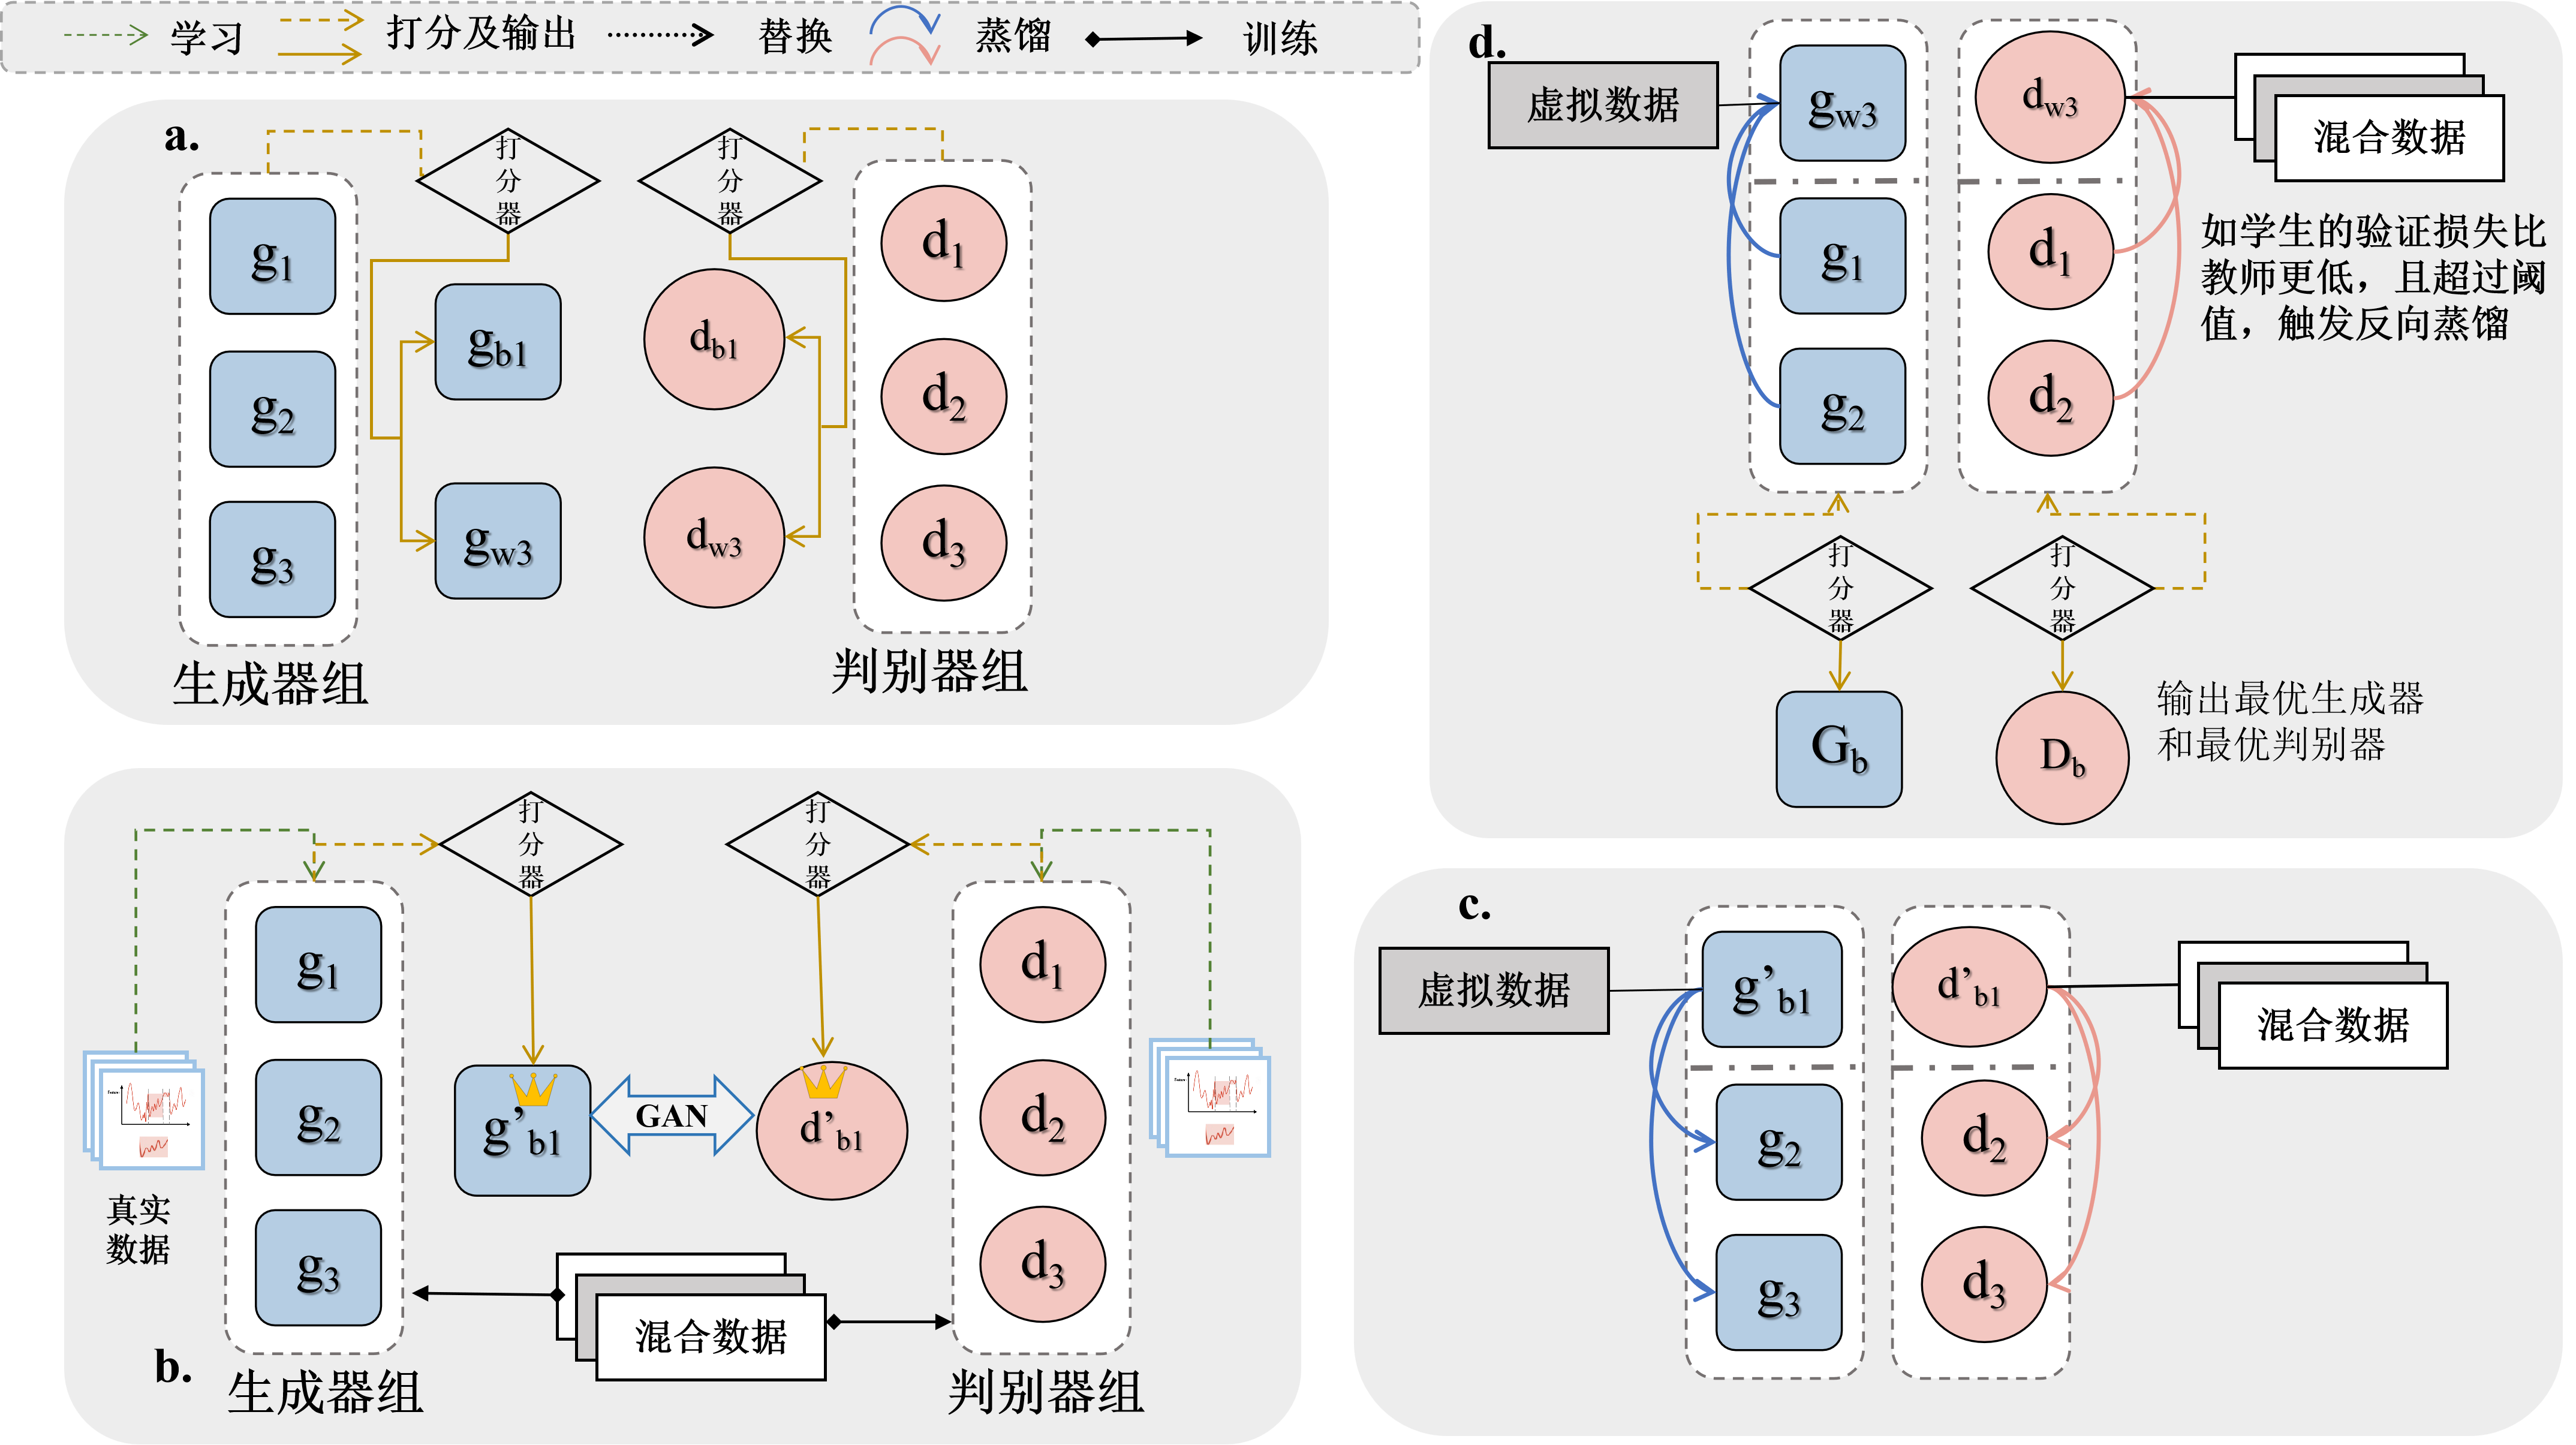
\includegraphics[width=0.8\textwidth]{figures/chap5/逆向对称.png}
    \caption{逆向师生蒸馏训练流程示意图}
    \label{fig:S2T-workflow}
\end{figure}

关于反馈阈值$\theta$的设定，本章采用动态自适应策略：以组内所有生成器在验证集上损失的均值$\bar{\mathcal{L}}$为基准，将阈值设定为$\theta = \alpha \cdot \bar{\mathcal{L}}$，其中$\alpha = 0.5$，即当最差成员的损失超过组内均值的1.5倍时触发蒸馏。在推理阶段，从训练完成后的生成器组中，选取在验证集上综合损失最小的生成器$G^\star_{\text{final}}$作为最终预测模型。这种动态阈值策略的优势在于：随着训练的推进，组内模型的整体损失逐渐降低，阈值也随之自适应调整，避免了固定阈值在训练早期过于宽松或后期过于严格的问题。

\subsection{带鱼短鱼机制趋势结构判别与策略映射}

本节进一步讨论时序结构识别结果如何转化为交易时机判断。四元分形事件用于描述结构事件是否出现，逆向师生蒸馏机制用于提升结构识别的稳定性，带鱼短鱼机制则用于判断已识别结构能否延续为具有交易意义的趋势波段。通过这一设计，本章将``结构是否出现''进一步转化为``结构是否具有交易意义''的判断，使模型输出能够服务后续交易执行优化与策略整合，并支撑交易流程中的交易时机判断。

在四元分形标签体系与逆向师生蒸馏机制的基础上，本章进一步引入``带鱼短鱼''机制，用于判断结构信号出现后能否延续为可交易的有效趋势。趋势跟随策略通常难以覆盖趋势启动初期的``鱼头''，也难以保留反转阶段的``鱼尾''，影响策略盈亏的关键，往往在于中段波段是否具有足够的延续性。基于这一考虑，本文将持续时间较长、终点价格优于起点价格的有效波段记为``带鱼''，将信号触发后较快反转、未形成有效收益的失败波段记为``短鱼''。其重点在于考察信号触发后的价格演化是否延续为有效趋势，而非评价信号形态本身是否完整。

这一划分为艾略特波浪理论中``有效浪''与``无效浪''的区分提供了可计算形式。将其纳入逆向师生蒸馏系统后，模型学习的对象不再只是局部结构是否出现，还包括该结构能否延续为有效趋势，从而为后续结构识别任务提供更稳定的监督信号。以指数平滑异同移动平均线金叉位置为波段起点 $t_s$，下一次反向信号（死叉）位置为波段终点 $t_e$，并以终点价格是否优于起点价格作为趋势有效性的判定准则：

\begin{equation}
\text{Label}_{[t_s, t_e]} =
\begin{cases}
\text{带鱼}, & \text{if } P_{t_e} > P_{t_s} \quad \text{（看涨波段）} \\
\text{短鱼}, & \text{if } P_{t_e} \leq P_{t_s} \quad \text{（看涨波段）}
\end{cases}
\end{equation}

对称地，在下跌趋势中：

\begin{equation}
\text{Label}_{[t_s, t_e]} =
\begin{cases}
\text{带鱼}, & \text{if } P_{t_e} < P_{t_s} \quad \text{（看跌波段）} \\
\text{短鱼}, & \text{if } P_{t_e} \geq P_{t_s} \quad \text{（看跌波段）}
\end{cases}
\end{equation}

这一机制可视为对四元分形事件划分的应用扩展。四元分形事件负责识别结构事件何时出现，``带鱼短鱼''则进一步判断这些结构是否真正转化为可持续的收益结构。若只看交叉或突破本身，模型容易学到大量假突破；而加入带鱼判定后，模型学习的对象同时包含``结构出现''与``结构是否走成''，从而更接近交易者真正关心的问题。

这一机制将``波段是否成功''转化为可观测、可训练的二元标签，解决了传统方法只能识别结构、不具备有效性验证机制的问题。从统计学角度来看，在本章所使用的15种期货品种的日频数据中，``短鱼''波段的数量通常占总波段数的60\%至75\%，呈现出典型的类别不平衡特征。这一分布特点进一步凸显了在模型训练中采用聚焦损失等不平衡处理策略的必要性。

从这一意义上看，本章最终形成的是一个“结构—有效性”两级标注框架：前层由 C/D/V/A 分形描述市场中的结构事件，后层由带鱼短鱼判定这些结构是否具备趋势持续性。这样处理既保留了波浪理论对结构的关注，也把无效信号过滤纳入可监督学习流程，为本章逆向师生蒸馏机制的训练与实验解释提供了更稳固的标签基础。更重要的是，该框架将``是否出现结构''与``是否值得据此交易''区分开来，使本章方法能够从结构识别进一步落到交易时机判断，而不是停留在一般分类任务。

\section{实验}

本章实验面向时序结构识别任务，检验逆向师生蒸馏学习方法在高噪声金融序列中是否能够提高结构事件识别的稳定性，并观察识别到的结构信号能否支撑交易时机判断。评价指标包括精确率、召回率、精确率与召回率调和平均值、混淆矩阵以及不同预训练模型对比，目的在于判断模型是否减少伪结构误判、保留有效结构信号，并为后续执行优化和策略整合提供更可靠的结构输入。因此，本章实验不是单纯比较分类器优劣，而是检验四元分形标注、逆向师生蒸馏和趋势有效性判别能否共同回应交易时机判断这一问题。

\subsection{实验数据集}
为验证基于四类分形模式的趋势识别方法及多智能体结构学习框架的有效性，本章选取中国商品期货市场具有代表性的15种主要期货品种作为研究对象，覆盖金属、农产品、能源化工及软商品等多个行业板块。数据集的构建目的在于检验模型对不同行情品种中时序结构的识别能力，因此实验不仅关注单个标签的分类结果，也关注结构事件在不同市场状态下的稳定性。所有数据均来自公开市场的日度行情，包含开盘价、最高价、最低价和收盘价等基础价格字段。本章进一步从开盘价、最高价、最低价和收盘价序列中构造短周期与长周期指数加权移动平均线（5指数加权移动平均线与120指数加权移动平均线）、价格变化率、实体宽度、上下影线比例等派生指标。在数据预处理阶段，首先剔除所有节假日与停牌日，对缺失数据点采用前向填充方式补全，并通过滑动窗口方式对部分派生特征进行平滑处理。四类分形结构标签基于本章提出的规则系统自动完成，最终形成的输入特征包含原始价格、技术指标、一阶变化率及多尺度结构信息。

\subsection{实验设计}
本章实验设计围绕两类目标展开：一是检验四元分形事件、逆向师生蒸馏机制与趋势有效性判别对时序结构识别稳定性的影响；二是说明这些结构信号能否服务于交易流程中的时机判断。因此，实验评价同时关注C/D/V/A四类结构事件的识别结果、不同模型预训练方式对结构边界的影响，以及逆向师生蒸馏机制对噪声误判和模式坍缩的缓解作用。

为保证实验结论能够同时反映识别性能与交易意义，本章在实验设计中同时设置结构事件识别评价和回测评价两个层次。其中，结构事件识别评价用于检验模型对C/D/V/A四类事件边界的识别能力，回测评价则用于检验上述结构事件是否能够进一步转化为交易时机判断。换言之，本节涉及的回测公式和交易指标属于实验设计中的验证口径，并不单独构成新的交易策略章节。

在特征工程层面，本章对输入特征进行了系统化的层次设计。第一层为基础价格特征，包括开盘价、最高价、最低价、收盘价四个原始字段；第二层为趋势敏感特征，包括5日指数加权移动平均线与120日指数加权移动平均线及其差值，用于捕捉短期与长期趋势的方向与强度；第三层为动量特征，包括指数平滑异同移动平均线的动量线、信号线与柱状线，以及价格的一阶变化率；第四层为K线结构特征，包括实体宽度（收盘价与开盘价之差的绝对值）、上影线长度、下影线长度及其比例关系。通过这种多层次的特征构建，模型能够同时获取价格的绝对水平、相对变化趋势、动量状态与微观结构信息，为后续的多任务学习提供了丰富的输入表示。

为量化评估四类分形结构标签体系与逆向师生蒸馏机制在实际交易中的表现，本章设计了基于日频价格序列的回测评估流程。策略每日仓位取值为+1（做多）、-1（做空）或0（中性/持有），由结构信号的预测方向直接决定。在单资产回测中，策略每日收益率计算方式为：

\begin{equation}
r_t^{\text{strategy}} = \text{pos}_{t-1} \cdot \left(\frac{P_t}{P_{t-1}} - 1\right) - \text{fee},
\end{equation}

其中$pos_{t-1}$为前一日仓位，$P_t$为第t日收盘价，fee为每笔交易的手续费。策略权益曲线以1.0为起点，通过逐日复利累乘计算：

\begin{equation}
\text{equity}_t = \prod_{i=1}^{t}\left(1 + r_i^{\text{strategy}}\right).
\end{equation}

本章采用以下评估指标：策略总累计收益率 $\text{TotalReturn} = \text{equity}_T - 1$；年化收益率 $\text{AnnualReturn} = \text{equity}_T^{252/T} - 1$；年化波动率 $\sigma_{\text{annual}} = \sqrt{252} \cdot \text{std}(\{r_t^{\text{strategy}}\})$；夏普比率 $\text{Sharpe} = (\bar{r}_{\text{annual}} - r_f) / \sigma_{\text{annual}}$；最大回撤 $\text{MDD} = \min_t\left(\text{equity}_t / \max_{i\le t}\text{equity}_i - 1\right)$；卡玛比率 $\text{Calmar} = \text{AnnualReturn} / |\text{MDD}|$。

在数据划分方面，本章采用时间序列的滚动窗口划分策略，以避免前视偏差。具体而言，将每个品种的历史数据按时间顺序划分为训练集（前60\%）、验证集（中间20\%）和测试集（后20\%）。验证集用于模型选择与超参数调优，测试集仅用于最终的性能评估与回测分析。所有评估指标均在测试集上计算，确保结果的客观性与可比性。

对比基线包括：GCA（多智能体对抗预训练模型）、GCA无内部知识共享版本（无内部知识共享的消融版本）、自注意力序列模型、门控循环单元、长短期记忆网络以及生成对抗网络六类具有代表性的预训练模型，涵盖生成式建模、序列建模与多智能体结构学习等不同范式。围绕分形事件识别任务（C、D、V、A），实验从两个层面评估模型的结构识别能力：一是逆向师生蒸馏机制与基线方法的总体比较，二是不同预训练模型对识别结果的影响。通过上述对比，可以观察逆向师生蒸馏机制在弱模型向强模型反向校正、波浪结构识别和局部伪结构过滤中的作用。

\subsection{结果分析与讨论}
本节从时序结构识别和交易时机判断两个层面解释实验结果。对于本章任务而言，准确率只能反映整体分类情况；精确率提升说明模型减少了伪结构误判，召回率提升说明模型能够捕捉更多真实结构事件，精确率与召回率调和平均值提升则说明模型在结构确认与信号覆盖之间取得更好平衡。对应到交易流程中，精确率关系到是否减少错误买入或错误卖出，召回率关系到是否遗漏有效趋势结构，因此这些指标共同反映了时序结构识别对交易时机判断的支持程度。

\begin{table}[htbp]
\centering
\caption{不同任务下基线方法与逆向师生蒸馏方法的性能对比}
\label{tab:s2t-performance}
\begin{tabular}{llcc}
\hline
\textbf{预测任务} & \textbf{指标} & \textbf{基线方法} & \textbf{逆向师生蒸馏机制} \\
\hline
\multirow{4}{*}{C} & 准确率  & 0.8814 & 0.8846 \\
                   & 精确率 & 0.2515 & 0.2572 \\
                   & 召回率    & 0.9498 & 0.9520 \\
                   & 精确率与召回率调和平均值        & 0.3977 & 0.4050 \\
\hline
\multirow{4}{*}{D} & 准确率  & 0.8859 & 0.9075 \\
                   & 精确率 & 0.2555 & 0.2920 \\
                   & 召回率    & 0.9138 & 0.8616 \\
                   & 精确率与召回率调和平均值        & 0.3994 & 0.4362 \\
\hline
\multirow{4}{*}{V} & 准确率  & 0.5664 & 0.4950 \\
                   & 精确率 & 0.4573 & 0.4242 \\
                   & 召回率    & 0.8175 & 0.9581 \\
                   & 精确率与召回率调和平均值        & 0.5865 & 0.5880 \\
\hline
\multirow{4}{*}{A} & 准确率  & 0.4724 & 0.4844 \\
                   & 精确率 & 0.4031 & 0.4082 \\
                   & 召回率    & 0.9555 & 0.9481 \\
                   & 精确率与召回率调和平均值        & 0.5670 & 0.5707 \\
\hline
\end{tabular}
\end{table}

从表\ref{tab:s2t-performance}与图\ref{fig:S2T-f1_bar}可以看出，逆向师生蒸馏机制在C与D两个方向切换类任务上均获得了稳定提升，其中D任务改善最为明显；在V与A任务中，模型则主要表现为召回率提升。这表明逆向师生蒸馏机制更有助于捕捉趋势切换与结构确认信号，同时在突破/跌破类事件中保留了更高的信号覆盖能力。图\ref{fig:S2T-cm_c}与图\ref{fig:S2T-cm_d}进一步给出了C、D任务的混淆矩阵结果，说明逆向师生蒸馏机制在关键时序结构识别中具有更好的判别效果；图\ref{fig:S2T-radarf1}则表明该优势具有一定的跨任务一致性。

\begin{figure}[htbp]
    \centering
    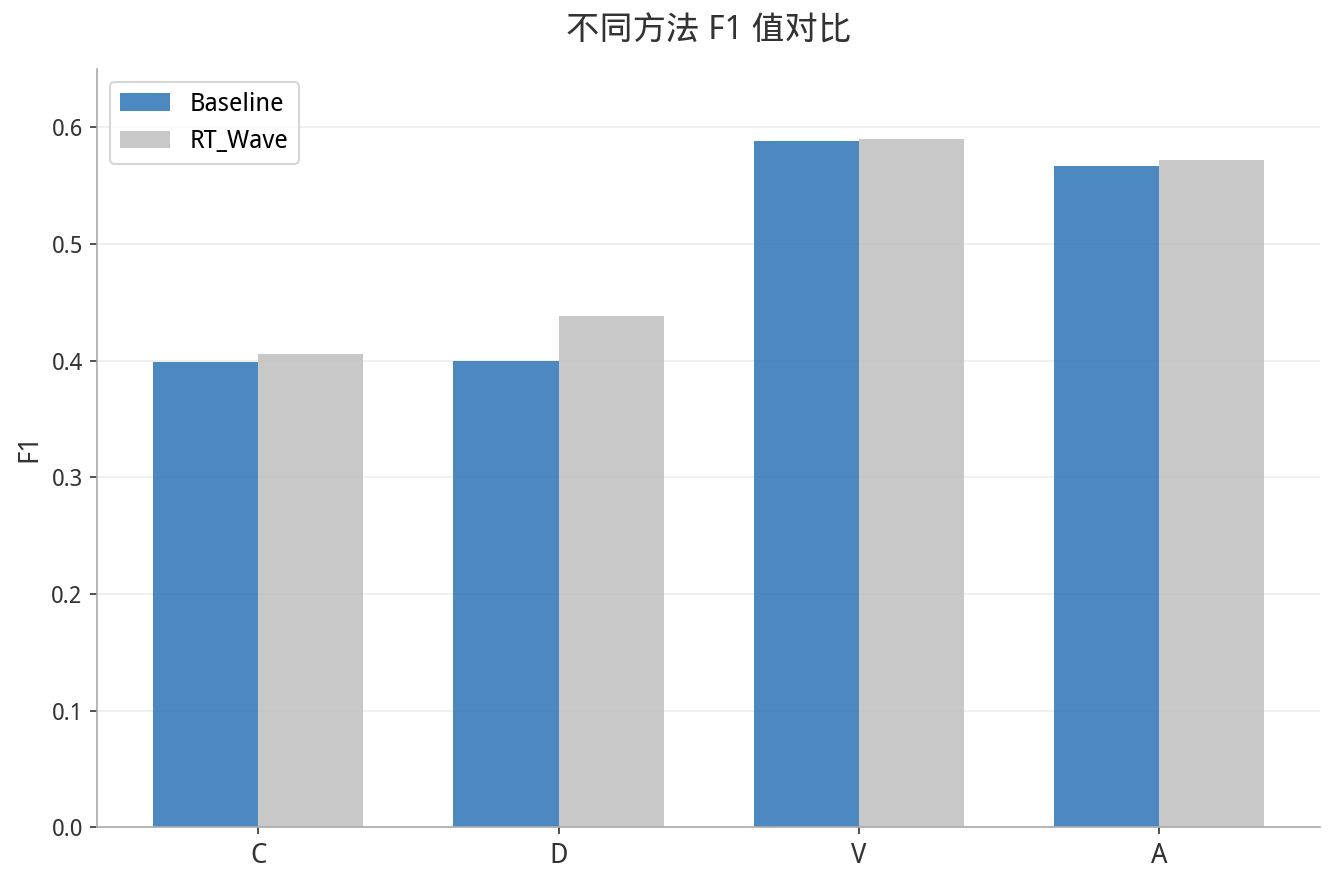
\includegraphics[width=1\linewidth]{figures/chap5/图4.5改.png}
    \caption{四类分形任务精确率与召回率调和平均值对比}
    \label{fig:S2T-f1_bar}
\end{figure}

\begin{figure}[htbp]
    \centering
    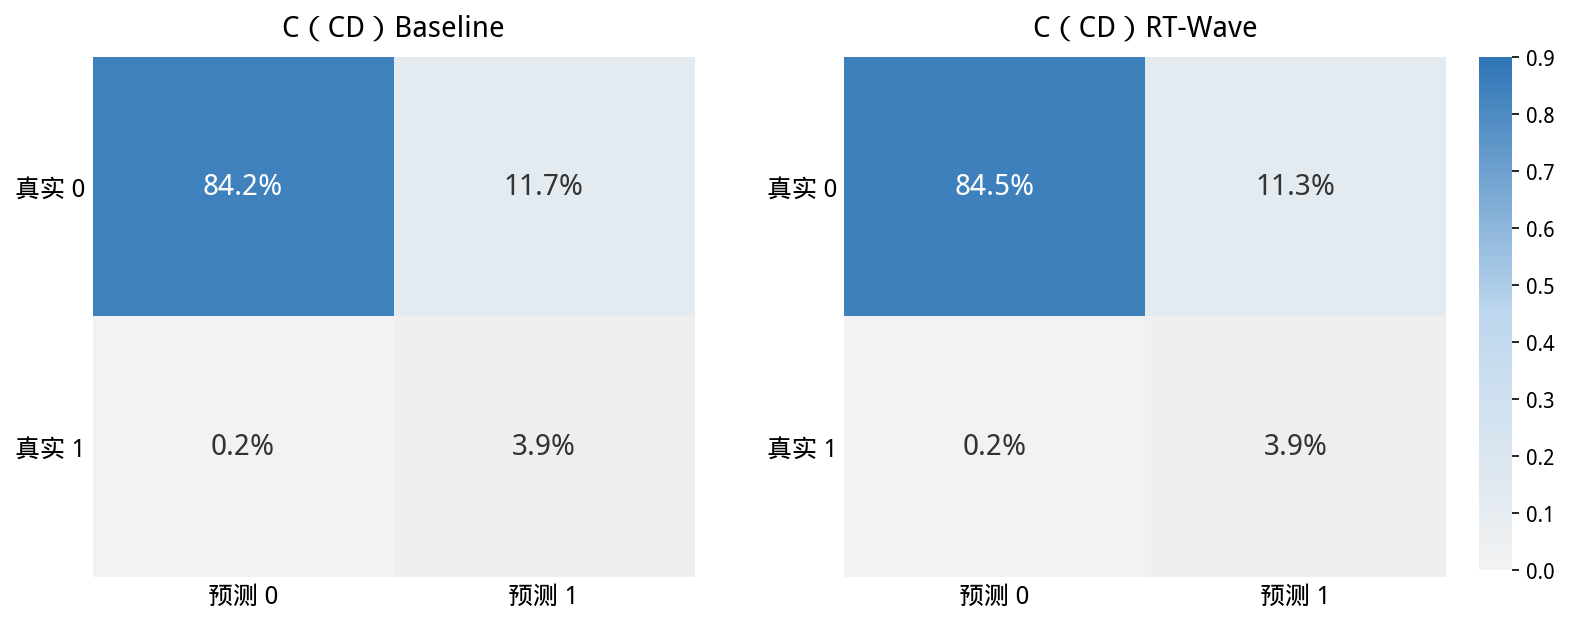
\includegraphics[width=1\linewidth]{figures/chap5/图4.6改.png}
    \caption{C 任务（看涨上穿）的混淆矩阵对比}
    \label{fig:S2T-cm_c}
\end{figure}

\begin{figure}[htbp]
    \centering
    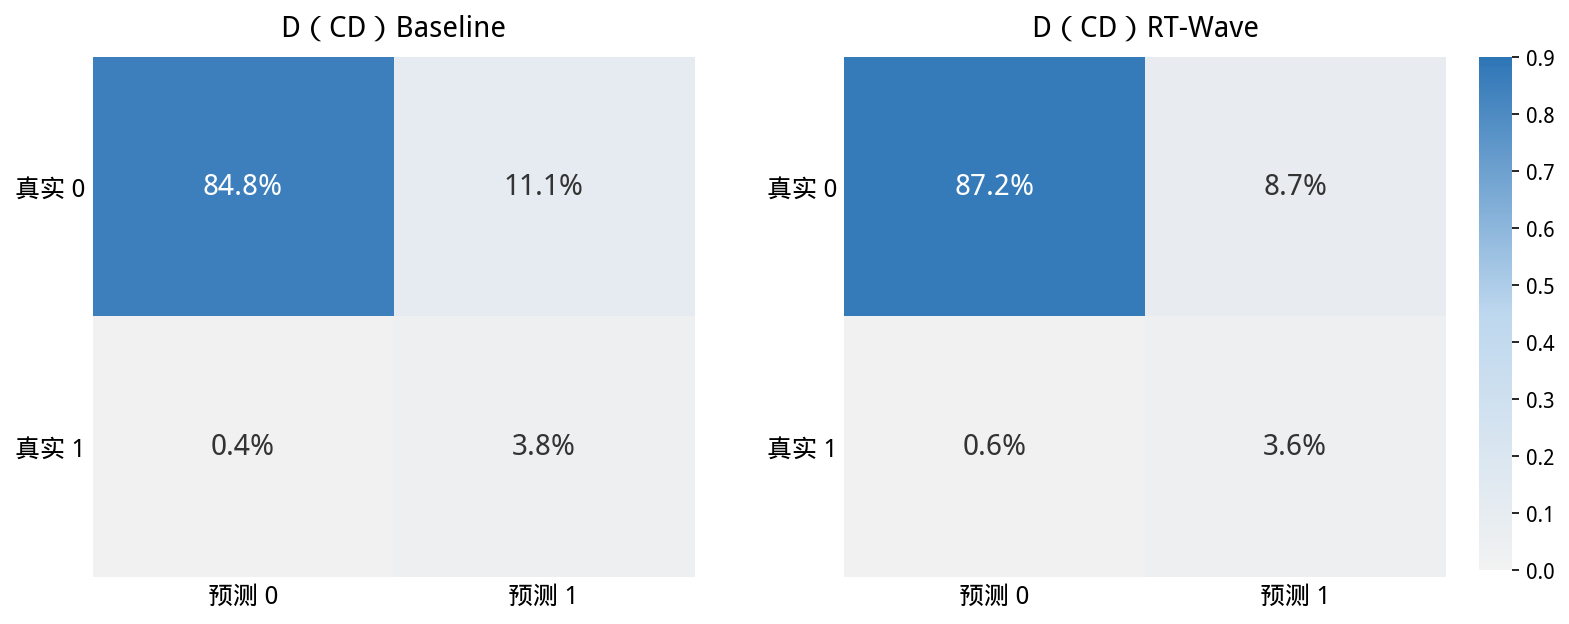
\includegraphics[width=1\linewidth]{figures/chap5/图4.7改.png}
    \caption{D 任务（看跌下穿）的混淆矩阵对比}
    \label{fig:S2T-cm_d}
\end{figure}

\begin{figure}[htbp]
    \centering
    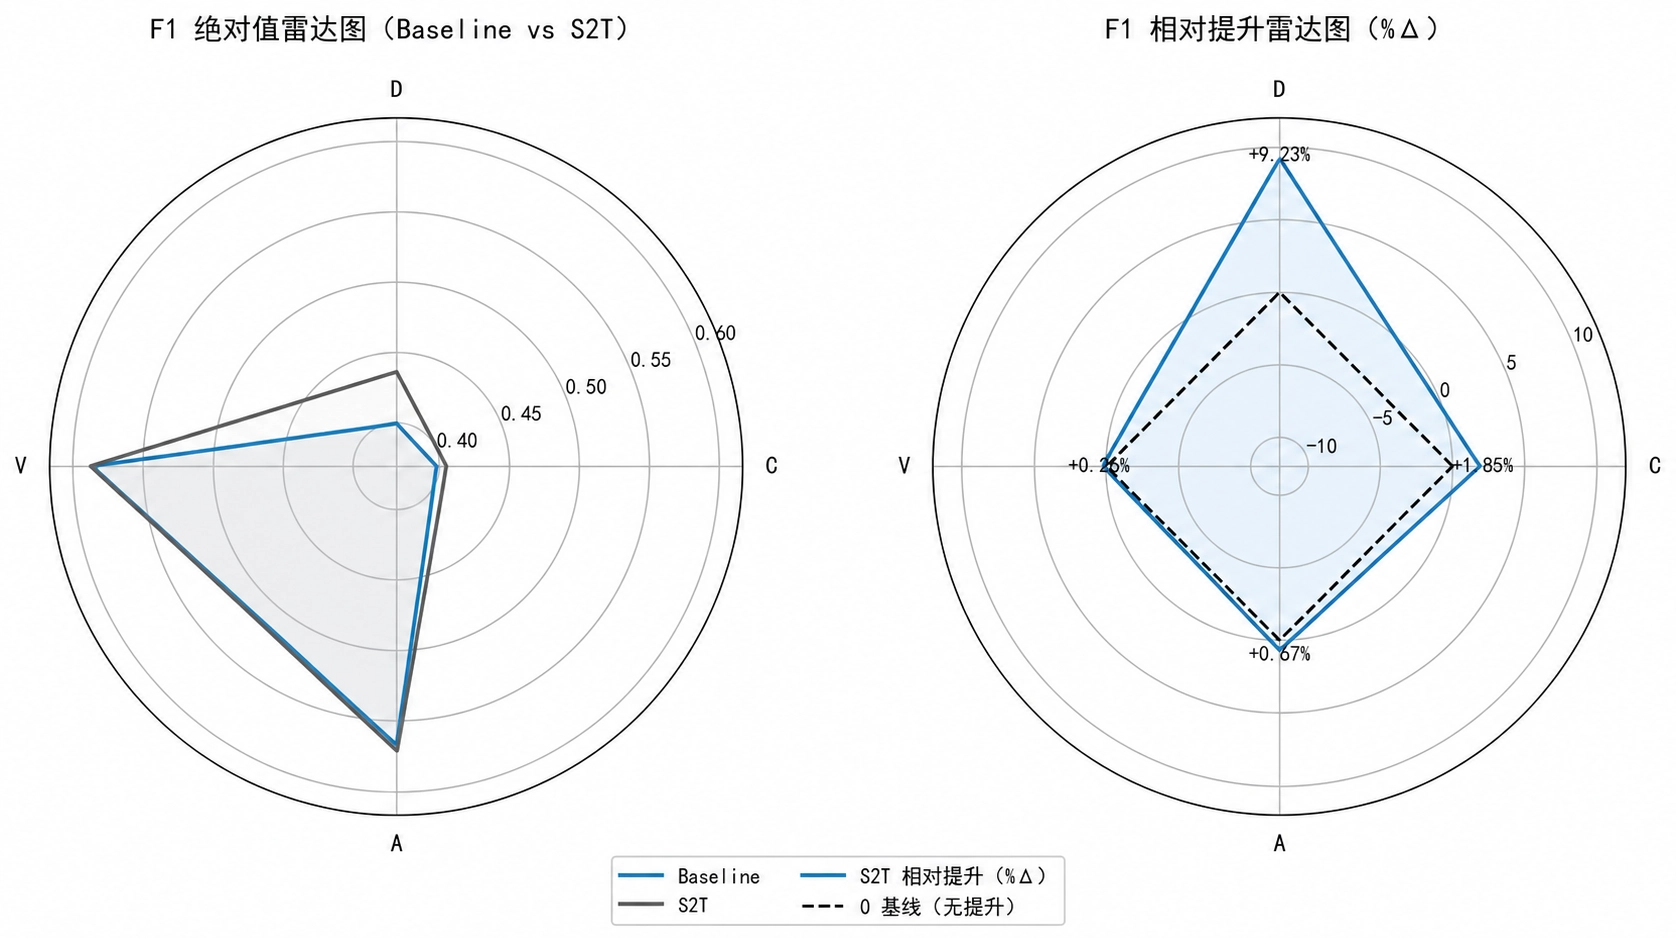
\includegraphics[width=1\linewidth]{figures/chap5/图4.8改.png}
    \caption{精确率与召回率调和平均值与相对提升雷达图}
    \label{fig:S2T-radarf1}
\end{figure}

\begin{figure}[htbp]
    \centering
    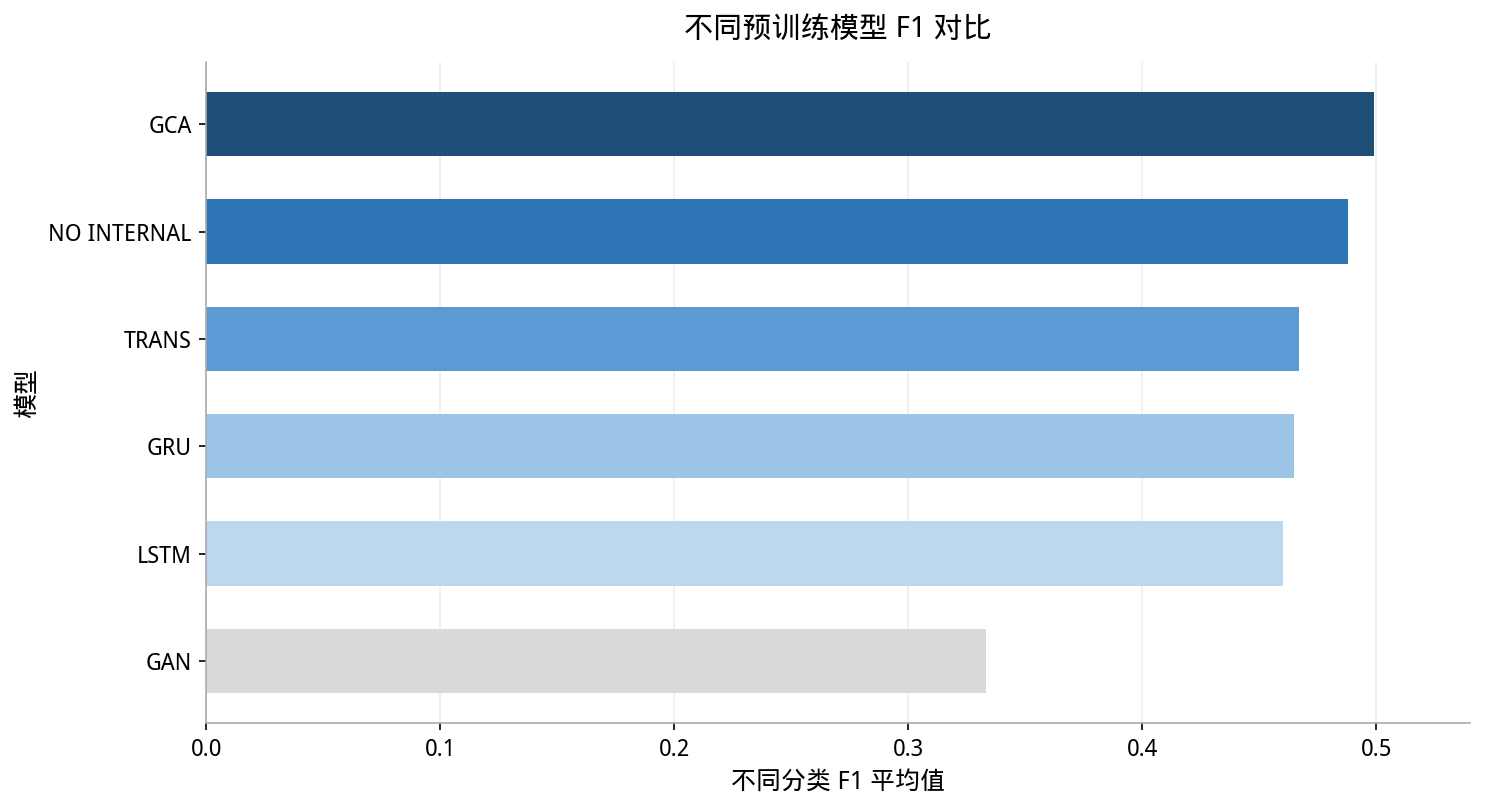
\includegraphics[width=1\linewidth]{figures/chap5/图4.9改.png}
    \caption{不同预训练模型平均精确率与召回率调和平均值对比图}
    \label{fig:S2T-models-F1}
\end{figure}

在预训练模型的对比实验中，从平均精确率与召回率调和平均值的柱状图\ref{fig:S2T-models-F1}可以看到，GCA在总体性能上位于最优水平，明显优于自注意力序列模型、门控循环单元、长短期记忆网络等常用时序模型，同时与GCA无内部知识共享版本拉开了可观察的差距。GCA无内部知识共享版本作为消融实验的对照组，移除了组内知识共享机制，其性能下降验证了多智能体内部协同对结构学习的贡献。进一步观察雷达图\ref{fig:S2T-models-radar}，GCA的优势具有明确的``结构一致性''特征：其在C与D两个方向切换类任务上呈现出更突出的精确率与召回率调和平均表现，同时在V与A两个突破/破位任务上也保持了相对更高且均衡的水平。相比之下，自注意力序列模型与长短期记忆网络虽然在部分任务上能够达到接近的精确率与召回率调和平均值，但在任务维度上呈现出更明显的``偏科''，导致整体平均效果无法超过GCA。

\begin{figure}[htbp]
    \centering
    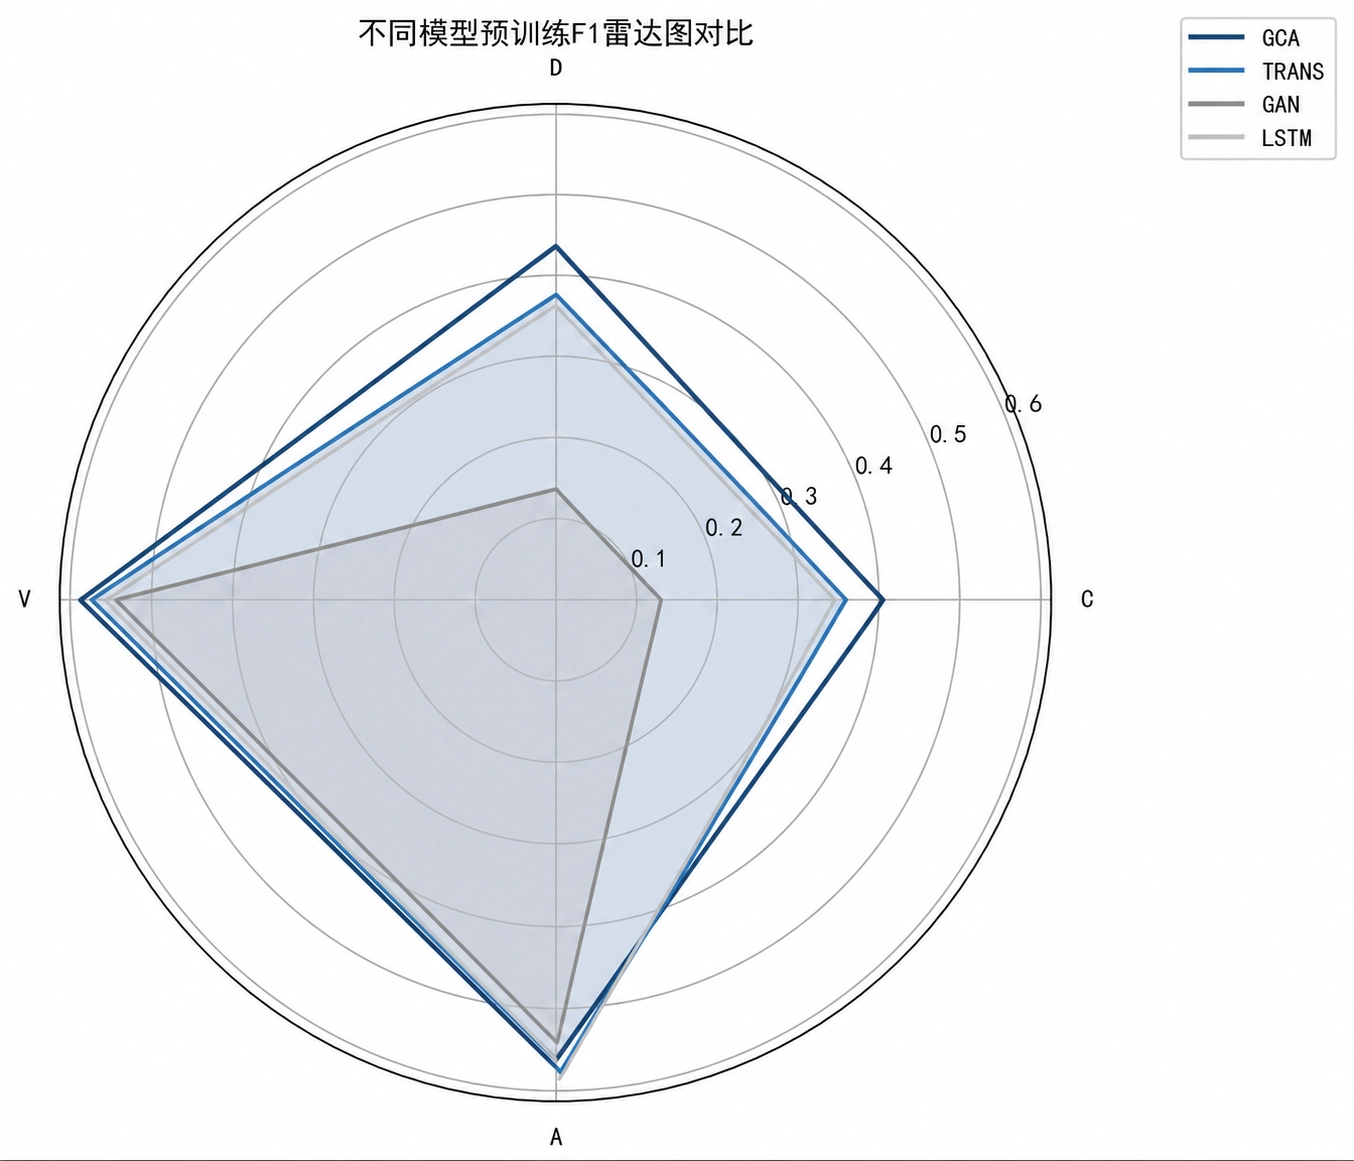
\includegraphics[width=0.75\linewidth]{figures/chap5/图4.10改.png}
    \caption{不同模型预训练精确率与召回率调和平均值对比雷达图}
    \label{fig:S2T-models-radar}
\end{figure}

\begin{figure}[htbp]
    \centering
    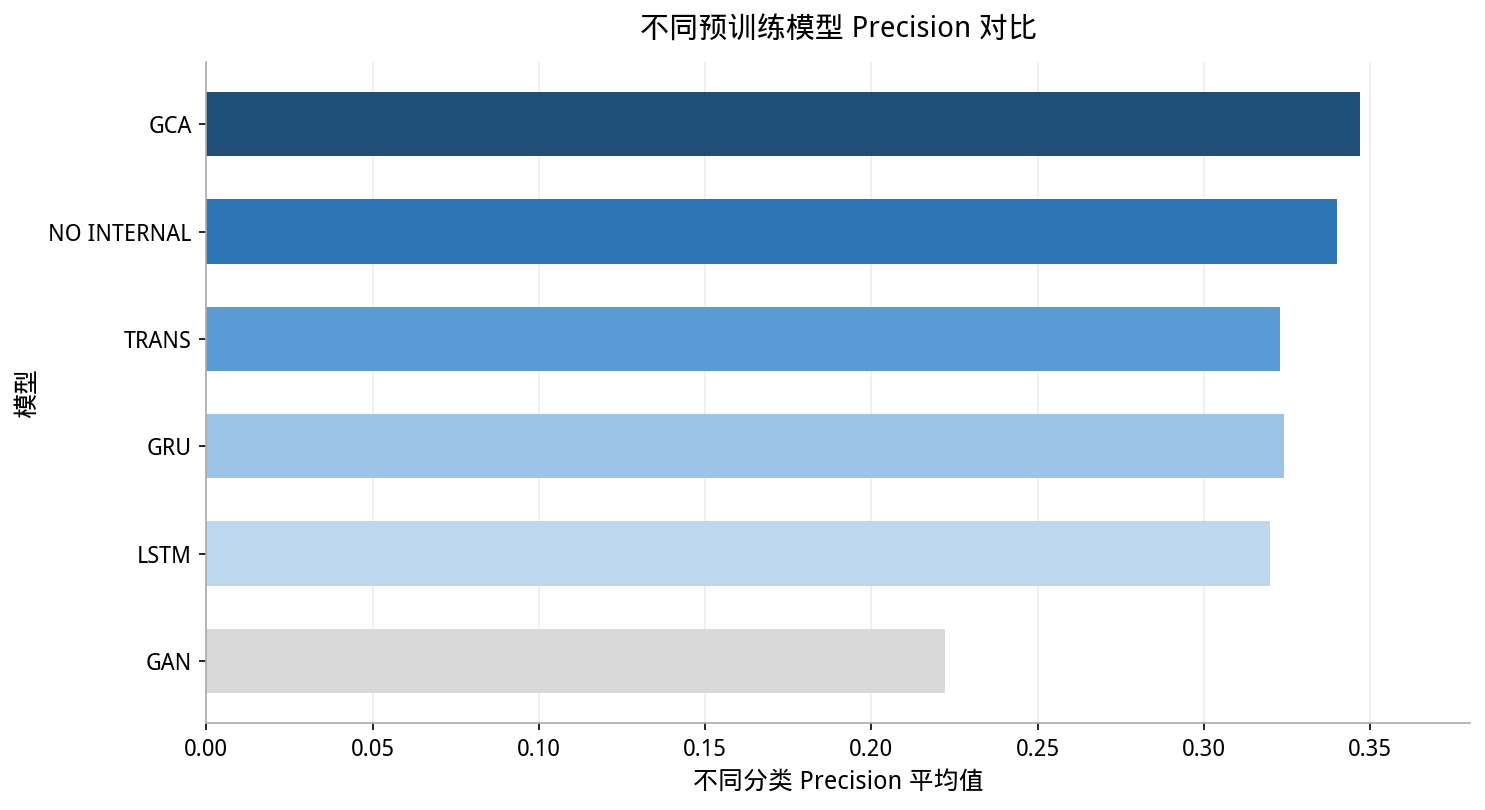
\includegraphics[width=0.75\linewidth]{figures/chap5/图4.11改.png}
    \caption{不同预训练模型平均精确率对比图}
    \label{fig:S2T-models-precision}
\end{figure}

\begin{figure}[htbp]
    \centering
    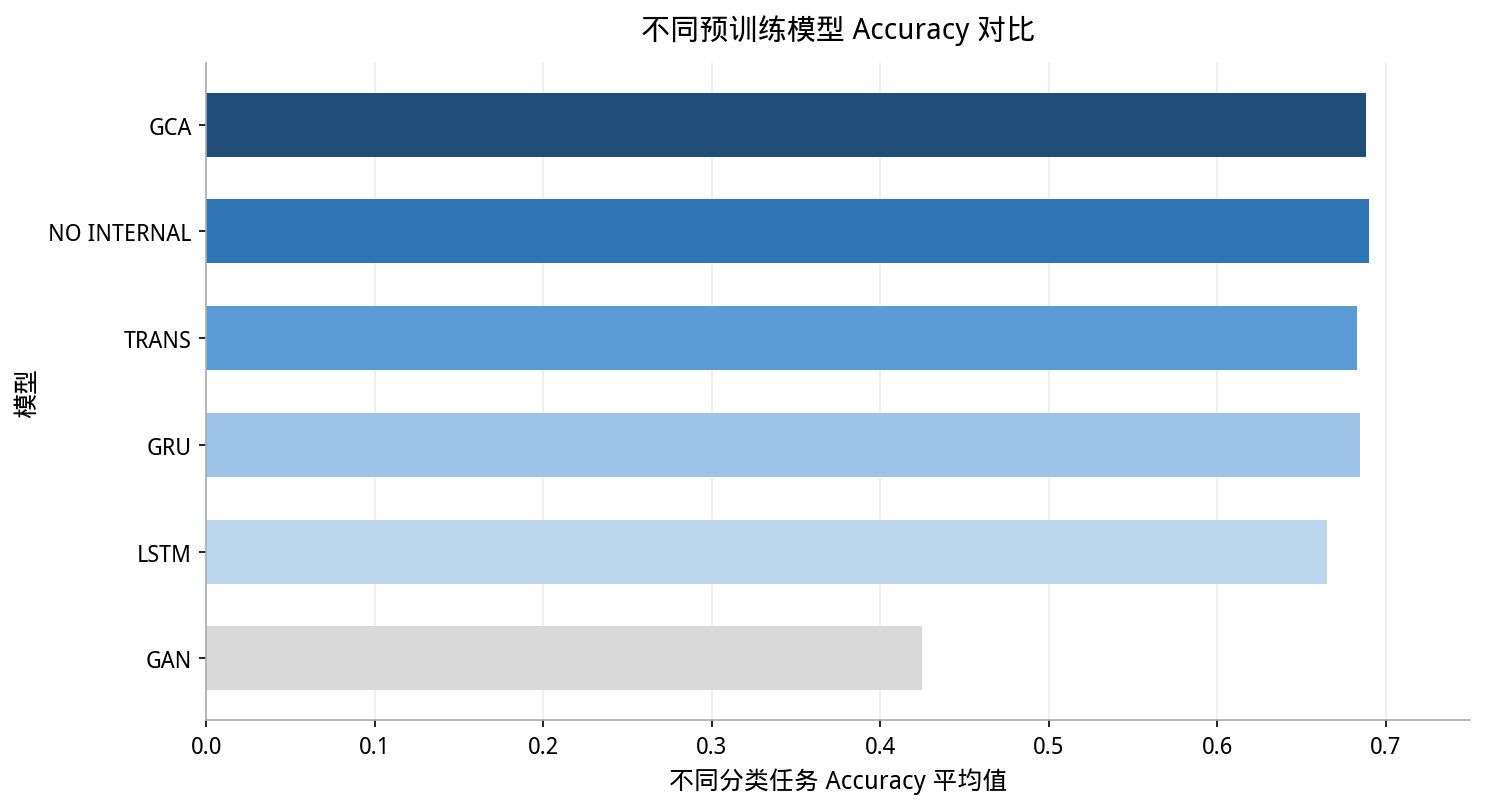
\includegraphics[width=0.75\linewidth]{figures/chap5/图4.12改.png}
    \caption{不同预训练模型平均准确率对比图}
    \label{fig:S2T-models-accuracy}
\end{figure}

图\ref{fig:S2T-models-precision}与图\ref{fig:S2T-models-accuracy}分别展示了不同预训练模型在平均精确率与平均准确率上的对比结果。整体来看，作为预训练配置的GCA在这两项指标上均保持较高水平，说明其在结构事件识别中具有较好的稳定性与均衡性。

本章实验显示，逆向师生蒸馏机制在部分任务上表现出相对优势。从知识蒸馏的理论视角来看，传统知识蒸馏可以看作一种相对静态的知识传递过程，学生模型被动拟合教师的平滑标签。而在金融时间序列这种极度非平稳、高噪声的环境中，固定的``强教师''极易对局部伪结构过拟合。逆向师生蒸馏机制对传统单向蒸馏方式作了调整，引入了由弱模型向强模型提供补充约束的训练机制。可以从训练过程的角度理解，这种机制可以理解为在多模型训练过程中引入了一种动态约束，使强模型在训练中参考弱模型所保留的较全局的结构信息，从而有助于缓解决策边界过于敏感以及模式坍缩问题。这与实验中D任务精确率从0.2555提升至0.2920的结果相吻合。

从金融分形结构的特征空间来看，四元分形事件在真实市场中呈现出典型的长尾分布与边界模糊性。逆向师生蒸馏机制通过多任务结构识别网络组的内部评分与交叉蒸馏，缓解模型在特征空间中过早趋同的问题。当最优模型试图利用特定的高频噪声捷径来降低训练损失时，逆向蒸馏促使其在训练中参考组内其他成员的分布信息，这种共识约束减弱了非平稳局部噪声带来的影响，学习到具有较强跨尺度稳定性的时序结构特征。此外，由于C/D分形依赖于指数平滑异同移动平均线等均线系统，该类标签在刻画市场结构时具有天然的滞后性偏差。本章通过引入基于K线实体突破的V/A信号，利用其价格行为的即时性对指数平滑异同移动平均线的滞后性进行补偿；同时，在多任务学习框架下，模型输入融合了多尺度特征与一阶动量变化率，使深度网络更可能学习到动量衰竭与结构反转的相关结构信息，这与由滞后识别向更早期结构判断的现象相一致。

从实验结果的局限性来看，V与A任务的精确率相对较低（均低于0.50），这反映了基于单根K线实体突破的V/A定义在高频场景下的固有噪声敏感性。具体而言，V任务的精确率从基线的0.4573下降至逆向师生蒸馏机制的0.4242，而召回率则从0.8175大幅提升至0.9581，这种精确率与召回率之间的权衡反映了逆向师生蒸馏机制在面对高频V/A事件时的策略倾向：模型更倾向于捕获尽可能多的真实结构信号，即使这意味着引入更多的假正例。在实际交易应用中，这种倾向可以通过后续的信号过滤模块加以修正，例如结合成交量确认或多周期一致性检验来剔除低置信度的V/A信号。

在消融实验的分析中，GCA无内部知识共享版本的性能下降幅度为理解模型内部协同机制的贡献提供了量化依据。移除组内知识共享后，模型在C任务上的精确率与召回率调和平均值下降约5\%，在D任务上下降约8\%，这一结果反映出组内蒸馏机制对于方向切换类事件的识别贡献相对更大。进一步分析发现，生成对抗网络基线模型在V/A任务上的表现相对较好，但在C/D任务上明显落后于GCA，这与生成对抗网络缺乏显式的结构化标签监督有关——生成对抗网络的生成器主要学习数据分布的整体统计特性，而非特定的结构转折模式。相比之下，GCA通过将对抗训练与结构化监督相结合，能够在保持分布拟合能力的同时增强对特定结构事件的判别精度。

从模型训练的收敛行为来看，逆向师生蒸馏机制在训练中期表现出一定的``震荡收敛''特征：由于反向蒸馏的周期性触发，强模型的验证损失可能出现短暂的上升波动，随后在正向蒸馏的驱动下重新下降。与传统单向蒸馏的单调收敛相比，这种训练扰动有助于缓解模型过早停留在局部最优附近的问题。在15个期货品种的实验中，约有11个品种在逆向师生蒸馏训练后期观察到了这种震荡收敛现象，且最终收敛值均低于未使用逆向师生蒸馏机制的对照组，进一步验证了反向蒸馏机制在优化景观中的探索作用。

在未来的工作中，可以考虑引入多周期确认机制或自适应阈值策略，以进一步提升V/A事件识别的精确率。此外，当前实验仅在日频数据上进行验证，将四元分形事件框架扩展至分钟级或tick级数据时，可能需要对分形事件的定义参数进行重新校准。另一个值得探索的方向是将四元分形标签体系与注意力可视化技术相结合，通过分析模型在做出结构识别决策时关注的时间窗口位置与特征维度，进一步提升框架的可解释性，为交易策略的设计提供更直观的依据。


\section{本章小结}

本章围绕对冲基金交易决策流程中的时序结构识别环节，提出面向时序结构识别的逆向师生蒸馏学习方法，重点服务于交易时机判断问题。与第2章侧重投资组合管理、第3章侧重高维金融因子建模不同，本章进一步关注价格路径中的趋势结构、结构边界与有效波段，尝试将传统波浪理论中的主观形态判断转化为可监督、可检验的时序结构识别任务。由此，波浪结构识别在本章中承担时序结构识别的具体实现功能，其目标是为后续交易执行优化和策略整合提供更可靠的结构信号。

在方法层面，本章工作主要体现在三个方面。第一，通过四元分形事件标注方法，将复杂的波浪形态量化为C、D、V、A四类结构事件，其中C/D基于指数平滑异同移动平均线动量指标捕捉宏观趋势转折，V/A基于K线实体突破捕捉微观结构波动，二者在时间尺度上形成互补，共同构成了面向时序结构识别的结构化标签体系。第二，逆向师生蒸馏机制对单向知识传递方式作了调整，通过动态监控与反向校正，使强模型在训练中参考弱模型保留的较全局结构信息，缓解多任务结构识别中的类别不平衡、局部伪结构过拟合与决策边界锐化问题。第三，引入``带鱼短鱼''机制对趋势的延续与反转提供较清晰的数学界定，将传统波浪理论中``有效浪''与``无效浪''的定性判断转化为基于价格终点与起点比较的二元判定，使模型能够进一步判断结构信号是否延续为具有交易意义的趋势波段。

在实验层面，本章在15种中国商品期货品种的日频数据上进行了验证。实验结果显示，逆向师生蒸馏机制在C与D两个核心任务上取得了稳定的精确率与召回率调和平均值提升，其中D任务的精确率与召回率调和平均值提升幅度超过9\%，精确率提升超过14\%。在预训练模型的对比实验中，作为预训练配置的GCA在平均精确率与召回率调和平均值、精确率与准确率三个维度上均优于自注意力序列模型、门控循环单元、长短期记忆网络等常用基线模型，说明协同训练在金融结构化建模中具有一定作用。混淆矩阵分析进一步揭示了逆向师生蒸馏机制在降低假正例率方面的优势，尤其在D任务中，模型对看跌结构转折的判别精度得到了实质性改善。上述结果说明，本章方法不仅改善了局部分类指标，也提高了时序结构信号对交易时机判断的支持能力。

尽管本章取得了一定的实验结果，但仍存在若干局限性与待改进之处。第一，V与A任务的精确率仍然偏低，这与基于单根K线实体突破的定义在高频场景下的固有噪声敏感性有关，未来可通过引入多周期确认机制或自适应阈值策略加以改善。第二，当前实验仅在日频数据上进行验证，将四元分形事件框架扩展至更高频率的数据时，分形事件的定义参数可能需要重新校准。第三，反向蒸馏的触发阈值目前采用的是基于组内均值的动态策略，未来可以探索更加精细化的自适应触发机制，例如基于梯度信息或特征空间多样性指标的动态调整策略。第四，本章主要关注结构识别性能指标，尚未将四元分形事件结构信号与实际交易策略的盈亏表现进行系统关联分析，这将在后续章节中通过交易执行优化与策略整合模块的结合加以完善。

本章对应交易决策链条中的第三个环节，即在明确资产配置和因子依据形成之后，判断交易时机判断。通过四元分形事件、逆向师生蒸馏机制和带鱼短鱼机制，本章形成了从结构事件标注、结构边界校正到趋势有效性判别的分析路径。第5章将在此基础上讨论结构信号确认后的交易执行路径优化，第6章则继续面向最终交易判断讨论策略整合问题。
